\documentclass[12pt,a4paper]{article}
\usepackage[utf8]{inputenc}
\usepackage{array}

\usepackage{geometry}
\usepackage{graphicx}
\usepackage{fancyhdr}
\usepackage{amsmath}
\usepackage{amsfonts}
\usepackage{amssymb}
\usepackage{color}
\usepackage{hyperref}
\usepackage{tikz}
\usetikzlibrary{shapes.geometric,arrows,positioning,shadows}
\usepackage{pgfgantt}
\usepackage{float}
\usepackage{listings}
\usepackage{xcolor}
\usepackage{booktabs}
\usepackage{multirow}
\usepackage{array}
\usepackage{subcaption}
\usepackage{titlesec}
\usepackage{multicol}
\usepackage{caption}
\usepackage{colortbl}
\usepackage{xcolor}
\usepackage{multirow}
\usepackage{array}

% Remove color styling that causes table issues
% Professional caption configuration - coordinated styling
\captionsetup{
    font={bf,small},
    textfont={color=bodytext},
    labelfont={color=primaryblue, bf},
    justification=centering,
    singlelinecheck=false,
    labelsep=period,
    skip=10pt,
    position=bottom
}

% Professional subcaption formatting - coordinated styling
\captionsetup[sub]{
    font={bf,footnotesize},
    textfont={color=bodytext},
    labelfont={color=secondaryblue, bf},
    justification=centering,
    singlelinecheck=false,
    labelsep=period,
    skip=8pt
}

% Professional table formatting with coordinated styling
\definecolor{tableheader}{RGB}{0,82,165}         % Primary blue for headers
\definecolor{tablebody}{RGB}{240,248,255}        % Very light blue
\definecolor{tableaccent}{RGB}{25,118,210}       % Secondary blue accent
\definecolor{tableborder}{RGB}{0,82,165}         % Primary blue border

% Additional color definitions for enhanced tables
\definecolor{headertext}{RGB}{255,255,255}       % White text for headers
\definecolor{bodytext}{RGB}{66,66,66}            % Professional dark gray
\definecolor{tablealt1}{RGB}{248,251,255}        % Alternating row color 1
\definecolor{tablealt2}{RGB}{235,245,251}        % Alternating row color 2
\definecolor{greentable}{RGB}{76,175,80}         % Professional green
\definecolor{orangetable}{RGB}{255,152,0}        % Professional orange
\definecolor{purpletable}{RGB}{156,39,176}       % Professional purple

% Enhanced table styling commands
\newcommand{\tableheaderrow}[1]{\rowcolor{tableheader}\textcolor{headertext}{\textbf{#1}}}
\newcommand{\tablealtrow}{\rowcolor{tablealt1}}
\newcommand{\tablealtrowtwo}{\rowcolor{tablealt2}}
\newcommand{\specialheader}[2]{\rowcolor{#1}\textcolor{headertext}{\textbf{#2}}}

% Set default array rule width for professional borders
\setlength{\arrayrulewidth}{1.2pt}

% Configure hyperref with professional colors
\hypersetup{
    colorlinks=true,
    linkcolor=primaryblue,
    filecolor=secondaryblue,      
    urlcolor=accentblue,
    pdftitle={Chapter 1: Introduction to Systems - Code Studio Software Company},
    pdfauthor={Sajidur Rahman Tarafder},
    pdfsubject={Systems Analysis and Design Lab Report}
}

% Enhanced code listings with professional colors
\lstset{
    basicstyle=\ttfamily\footnotesize,
    backgroundcolor=\color{lightgray},
    frame=leftline,
    framerule=3pt,
    rulecolor=\color{primaryblue},
    breaklines=true,
    captionpos=b,
    numbers=left,
    numberstyle=\tiny\color{darkgray}\bfseries,
    stepnumber=1,
    numbersep=12pt,
    keywordstyle=\color{primaryblue}\bfseries,
    commentstyle=\color{mediumgray}\itshape,
    stringstyle=\color{secondaryblue},
    emphstyle=\color{accentblue}\bfseries,
    showstringspaces=false,
    tabsize=2,
    xleftmargin=20pt,
    framexleftmargin=15pt,
    numberbychapter=false,
    firstnumber=1
}

% ===================== PROFESSIONAL COLOR SCHEME =====================
% Define professional color palette
\definecolor{primaryblue}{RGB}{0,82,165}        % Deep professional blue
\definecolor{secondaryblue}{RGB}{25,118,210}    % Medium blue
\definecolor{accentblue}{RGB}{100,181,246}      % Light blue accent
\definecolor{lightblue}{RGB}{173,216,230}       % Light blue for backgrounds
\definecolor{darkgray}{RGB}{66,66,66}           % Professional dark gray
\definecolor{mediumgray}{RGB}{117,117,117}      % Medium gray
\definecolor{lightgray}{RGB}{238,238,238}       % Light gray for backgrounds

% Professional section formatting with modern styling
\titleformat{\section}[hang]
{\normalfont\LARGE\bfseries\color{primaryblue}}
{\colorbox{primaryblue}{\makebox[1.8em]{\textcolor{white}{\thesection}}}~}{0.5em}
{}
[\vspace{2pt}{\color{primaryblue}\hrule height 1pt width \textwidth}]
\titlespacing*{\section}{0pt}{25pt}{18pt}

% Professional subsection formatting with perfect left alignment
\titleformat{\subsection}[block]
{\normalfont\Large\bfseries\color{secondaryblue}}
{\thesubsection.~}{0pt}
{}
[\vspace{1pt}{\color{secondaryblue}\hrule height 0.8pt width \textwidth}]
\titlespacing*{\subsection}{0pt}{20pt}{14pt}

% Modern subsubsection formatting with perfect left alignment
\titleformat{\subsubsection}[block]
{\normalfont\large\bfseries\color{accentblue}}
{\thesubsubsection.~}{0pt}
{}
[\vspace{0.5pt}{\color{accentblue}\hrule height 0.5pt width \textwidth}]
\titlespacing*{\subsubsection}{0pt}{15pt}{10pt}

% Define custom project title formatting (left-aligned with consistent underlines)
\newcommand{\projecttitle}[1]{%
    \vspace{15pt}%
    \noindent{\normalfont\Large\bfseries\color{accentblue}#1}%
    \vspace{1pt}\noindent{\color{accentblue}\hrule height 0.8pt width \textwidth}%
    \vspace{10pt}%
}

% ===================== PROFESSIONAL HEADER SETUP =====================
% Configure geometry for header space
\geometry{
    top=2.5cm,
    bottom=2.5cm,
    left=2.5cm,
    right=2.5cm,
    headheight=25pt,
    headsep=30pt
}

% Professional header and footer design
\fancypagestyle{reportstyle}{%
    \fancyhf{}% Clear all headers and footers
    
    % Header setup
    \fancyhead[L]{\textcolor{primaryblue}{\textbf{CSE 4120 - Final Lab Report}}}
    \fancyhead[R]{\textcolor{primaryblue}{\textbf{Customer Segmentation Classification}}}
    
    % Header line
    \renewcommand{\headrulewidth}{1pt}
    \renewcommand{\headrule}{\hbox to\headwidth{%
        \color{primaryblue}\leaders\hrule height \headrulewidth\hfill}}
    
    % Footer setup - only page number
    \fancyfoot[C]{\textcolor{primaryblue}{\textbf{\thepage}}}
    
    % No footer line
    \renewcommand{\footrulewidth}{0pt}
}

% Chapter 2 page style
\fancypagestyle{chapter2style}{%
    \fancyhf{}
    
    % Header setup
    \fancyhead[L]{\textcolor{primaryblue}{\textbf{CSE 4120 - Data Mining Sessional}}}
    \fancyhead[R]{\textcolor{primaryblue}{\textbf{Customer Segmentation Analysis}}}
    
    % Header line
    \renewcommand{\headrulewidth}{1pt}
    \renewcommand{\headrule}{\hbox to\headwidth{%
        \color{primaryblue}\leaders\hrule height \headrulewidth\hfill}}
    
    % Footer setup - only page number
    \fancyfoot[C]{\textcolor{primaryblue}{\textbf{\thepage}}}
    
    % No footer line
    \renewcommand{\footrulewidth}{0pt}
}

% Chapter 3 page style
\fancypagestyle{chapter3style}{%
    \fancyhf{}
    
    % Header setup
    \fancyhead[L]{\textcolor{primaryblue}{\textbf{CSE 4120 - Data Mining Sessional}}}
    \fancyhead[R]{\textcolor{primaryblue}{\textbf{Customer Segmentation Analysis}}}
    
    % Header line
    \renewcommand{\headrulewidth}{1pt}
    \renewcommand{\headrule}{\hbox to\headwidth{%
        \color{primaryblue}\leaders\hrule height \headrulewidth\hfill}}
    
    % Footer setup - only page number
    \fancyfoot[C]{\textcolor{primaryblue}{\textbf{\thepage}}}
    
    % No footer line
    \renewcommand{\footrulewidth}{0pt}
}

% Title page style (no header/footer)
\fancypagestyle{titlepage}{%
    \fancyhf{}%
    \renewcommand{\headrulewidth}{0pt}%
    \renewcommand{\footrulewidth}{0pt}%
}

% Set default page style after title page
% ===================== ENHANCED STYLING =====================

\begin{document}

% ===================== COVER PAGE =====================

\begin{titlepage}
    \thispagestyle{empty}
    \centering
    \vspace*{0.5cm}
    
    % University motto
    {\large \textbf{"Heaven's Light is Our Guide"}}\\[0.3cm]
    
    % University logo
    \includegraphics[width=4cm]{ruet_logo.png} \\[0.4cm]
    
    % University name
    {\Large \textbf{Department of Computer Science \& Engineering}}\\[0.3cm]
    {\large \textbf{Rajshahi University of Engineering \& Technology}}\\[0.8cm]

    \vspace{0.8cm}
    % Report title
    {\LARGE \textbf{Final Lab Report}}\\[0.4cm]

    \vspace{0.8cm}
    % Course details
    {\Large \textbf{Course Code: CSE 4120}}\\[0.3cm]
    {\Large \textbf{Course Title: Data Mining Sessional}}\\[0.4cm]
    {\LARGE \textbf{Customer Segmentation Classification}}\\[0.8cm]
    
    
    % Submission details table with proper formatting
    \begin{table}[h!]
    \centering
    \setlength{\arrayrulewidth}{1.5pt}
    \renewcommand{\arraystretch}{1.5}
    \begin{tabular}{|p{8.5cm}|p{6.5cm}|}
        \hline
        \multicolumn{1}{|c|}{\large \textbf{Submitted By:}} & \multicolumn{1}{c|}{\large \textbf{Submitted To:}} \\
        \hline
        & \\
        \large \textbf{Name: Sajidur Rahman Tarafder} & \multirow{5}{*}{\parbox{6.5cm}{\centering 
        \large \textbf{Julia Rahman} \\ 
        \vspace{0.2cm}
        \large \textbf{Associate Professor} \\ 
        \vspace{0.2cm}
        \large \textbf{Department of CSE RUET} \\ 
        \vspace{0.4cm}}} \\
        \large \textbf{Roll: 2003154} & \\
        \large \textbf{Section: C} & \\
        \large \textbf{Session: 2020-21} & \\
        \large \textbf{Department: CSE} & \\
        & \\
        \hline
    \end{tabular}
    \end{table}
    
    \vspace{0.5cm}
\end{titlepage}

% Set page style for the document
\pagestyle{reportstyle}

\newpage

% ===================== TABLE OF CONTENTS =====================
% Remove numbering from table of contents
\renewcommand{\contentsname}{Table of Contents}
\setcounter{tocdepth}{3}
\makeatletter
\renewcommand{\l@section}{\@dottedtocline{1}{0em}{1.5em}}
\renewcommand{\l@subsection}{\@dottedtocline{2}{1.5em}{2.3em}}
\renewcommand{\l@subsubsection}{\@dottedtocline{3}{3em}{3.2em}}
\makeatother

\tableofcontents
\newpage

% ===================== INTRODUCTION =====================
\section{Introduction}

Customer segmentation represents one of the most critical applications in modern business analytics, enabling organizations to understand their diverse customer base through systematic data analysis. This comprehensive study explores the application of various data mining methodologies to uncover hidden patterns within customer behavior and demographics.

\subsection{Dataset Overview}

This analysis utilizes the Customer Segmentation Classification dataset, a comprehensive collection of customer information designed for machine learning and data mining applications. The dataset is publicly available on Kaggle and can be accessed at:\\

\textbf{Dataset:} https://www.kaggle.com/datasets/kaushiksuresh147/customer-segmentation

\subsubsection{Dataset Characteristics}

The dataset contains \textbf{8,068 customer records} with \textbf{11 distinct attributes}, providing a rich foundation for analytical exploration. The data encompasses both demographic and behavioral characteristics, creating a multifaceted view of customer profiles suitable for various data mining techniques.

\subsubsection{Feature Description}

The dataset includes the following key attributes:

\begin{itemize}
    \item \textbf{ID}: Unique customer identifier (Integer)
    \item \textbf{Gender}: Customer gender classification (Male/Female)
    \item \textbf{Ever\_Married}: Marital status indicator (Yes/No)
    \item \textbf{Age}: Customer age in years (Integer, 22-67 range observed)
    \item \textbf{Graduated}: Educational attainment indicator (Yes/No)
    \item \textbf{Profession}: Professional category (Healthcare, Engineer, Lawyer, Entertainment, etc.)
    \item \textbf{Work\_Experience}: Years of professional experience (Float, with some missing values)
    \item \textbf{Spending\_Score}: Customer spending behavior classification (Low/Average/High)
    \item \textbf{Family\_Size}: Number of family members (Float, 1.0-6.0 range observed)
    \item \textbf{Var\_1}: Additional categorical variable (Cat\_4, Cat\_6, etc.)
    \item \textbf{Segmentation}: Target variable with four customer segments (A, B, C, D)
\end{itemize}

% ===================== MODULE 1: DATA LOADING AND ANALYSIS =====================
\section{Introduction to Data Mining Tools}

\subsection{Dataset Loading from CSV/XLSX Format}

\subsubsection{Implementation Approach}
I loaded the Customer Segmentation Classification dataset using pandas to read the CSV file. I chose pandas because it provides powerful data manipulation capabilities and seamlessly handles CSV files. My approach involved importing essential libraries like pandas for data handling, numpy for numerical operations, matplotlib for visualization, and sklearn for machine learning tasks. 

\subsubsection{Implementation Code}
\begin{lstlisting}[language=Python, caption=Dataset Loading from CSV/XLSX Format]
# Importing necessary libraries
import pandas as pd
import numpy as np
import matplotlib.pyplot as plt
from sklearn.model_selection import train_test_split

print("Libraries imported successfully!")
# Loading the dataset
df = pd.read_csv('Customer_Segmentation_Classification.csv')
print("Loaded Customer_Segmentation_Classification.csv successfully!")
\end{lstlisting}

\subsubsection{Terminal Output}

\begin{figure}[h!]
\centering
    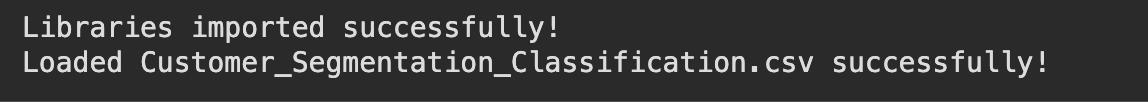
\includegraphics[width=\textwidth]{Figures/dataset_loading_output.png}
    \caption{Dataset Loaded Successfully}
    \label{fig:dataset_loading}
\end{figure}

\subsection{Data Type and Dimensionality Analysis}

\subsubsection{Implementation Approach}
I examined the dataset structure by checking its dimensions, data types, and basic information to understand the nature of the data I was working with. My strategy was to get a comprehensive overview of the dataset before diving into analysis. I used the shape attribute to determine the number of rows and columns, printed the column names to see what features were available, and checked data types using dtypes to identify which columns contained numerical versus categorical data. This initial exploration helped me plan my preprocessing and analysis approach effectively.

\subsubsection{Implementation Code}
\begin{lstlisting}[language=Python, caption=Data Type Analysis and Dimension Determination]
print(f"Dataset dimensions: {df.shape}")
print(f"Columns: {df.columns.tolist()}")
print(f"Data types:")
print(df.dtypes)
\end{lstlisting}

\subsubsection{Terminal Output}

\begin{figure}[h!]
\centering
    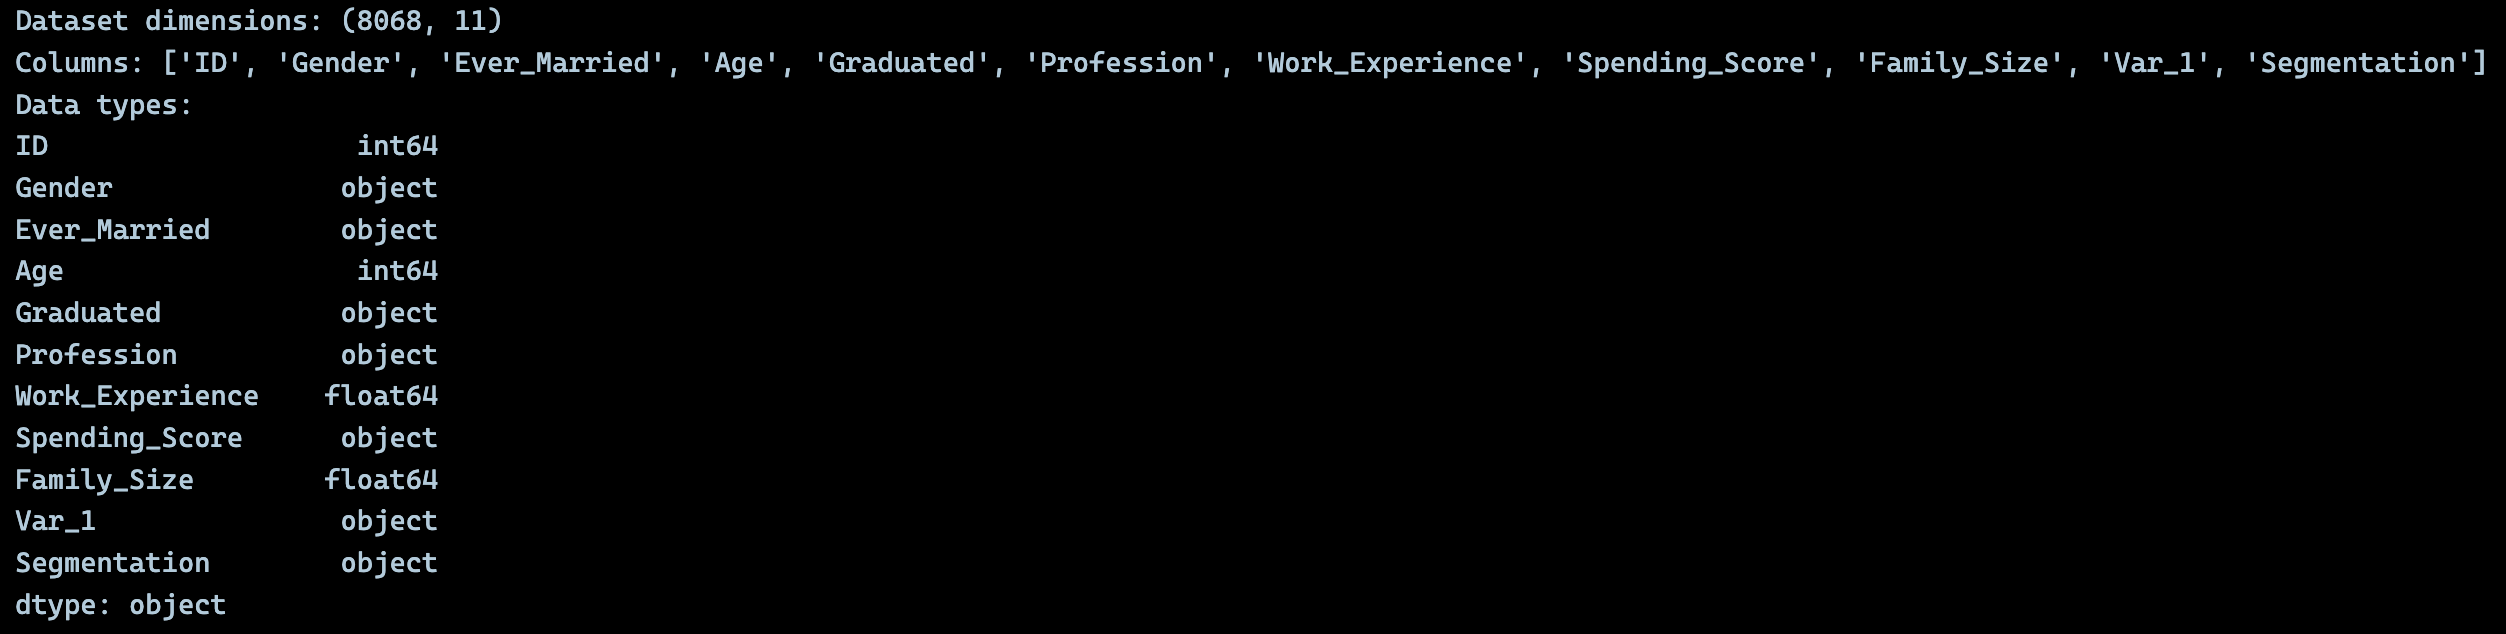
\includegraphics[width=\textwidth]{Figures/dataset_info_summary.png}
    \caption{Data Type and Dimensionality Analysis}
    \label{fig:dataset_info}
\end{figure}

\subsection{Labeled Column Identification}

\subsubsection{Implementation Approach}
I examined all columns to identify which one could serve as the target variable for prediction purposes. My approach involved inspecting the first few rows using head() to understand the data structure and then identifying the last column as the potential target variable. I printed the unique values in this column to see what categories or classes existed in the target variable. This step was crucial because understanding the target variable would determine whether this was a classification or regression problem and guide my subsequent modeling choices.

\subsubsection{Implementation Code}
\begin{lstlisting}[language=Python, caption=Labeled Column Identification]
# Potential labeled columns
print("First few rows:")
print(df.head())
print(f"\nPotential label column: {df.columns[-1]}")
print(f"Unique values in label: {df[df.columns[-1]].unique()}")
\end{lstlisting}

\newpage
\subsubsection{Terminal Output}
\begin{figure}[h!]
    \centering
    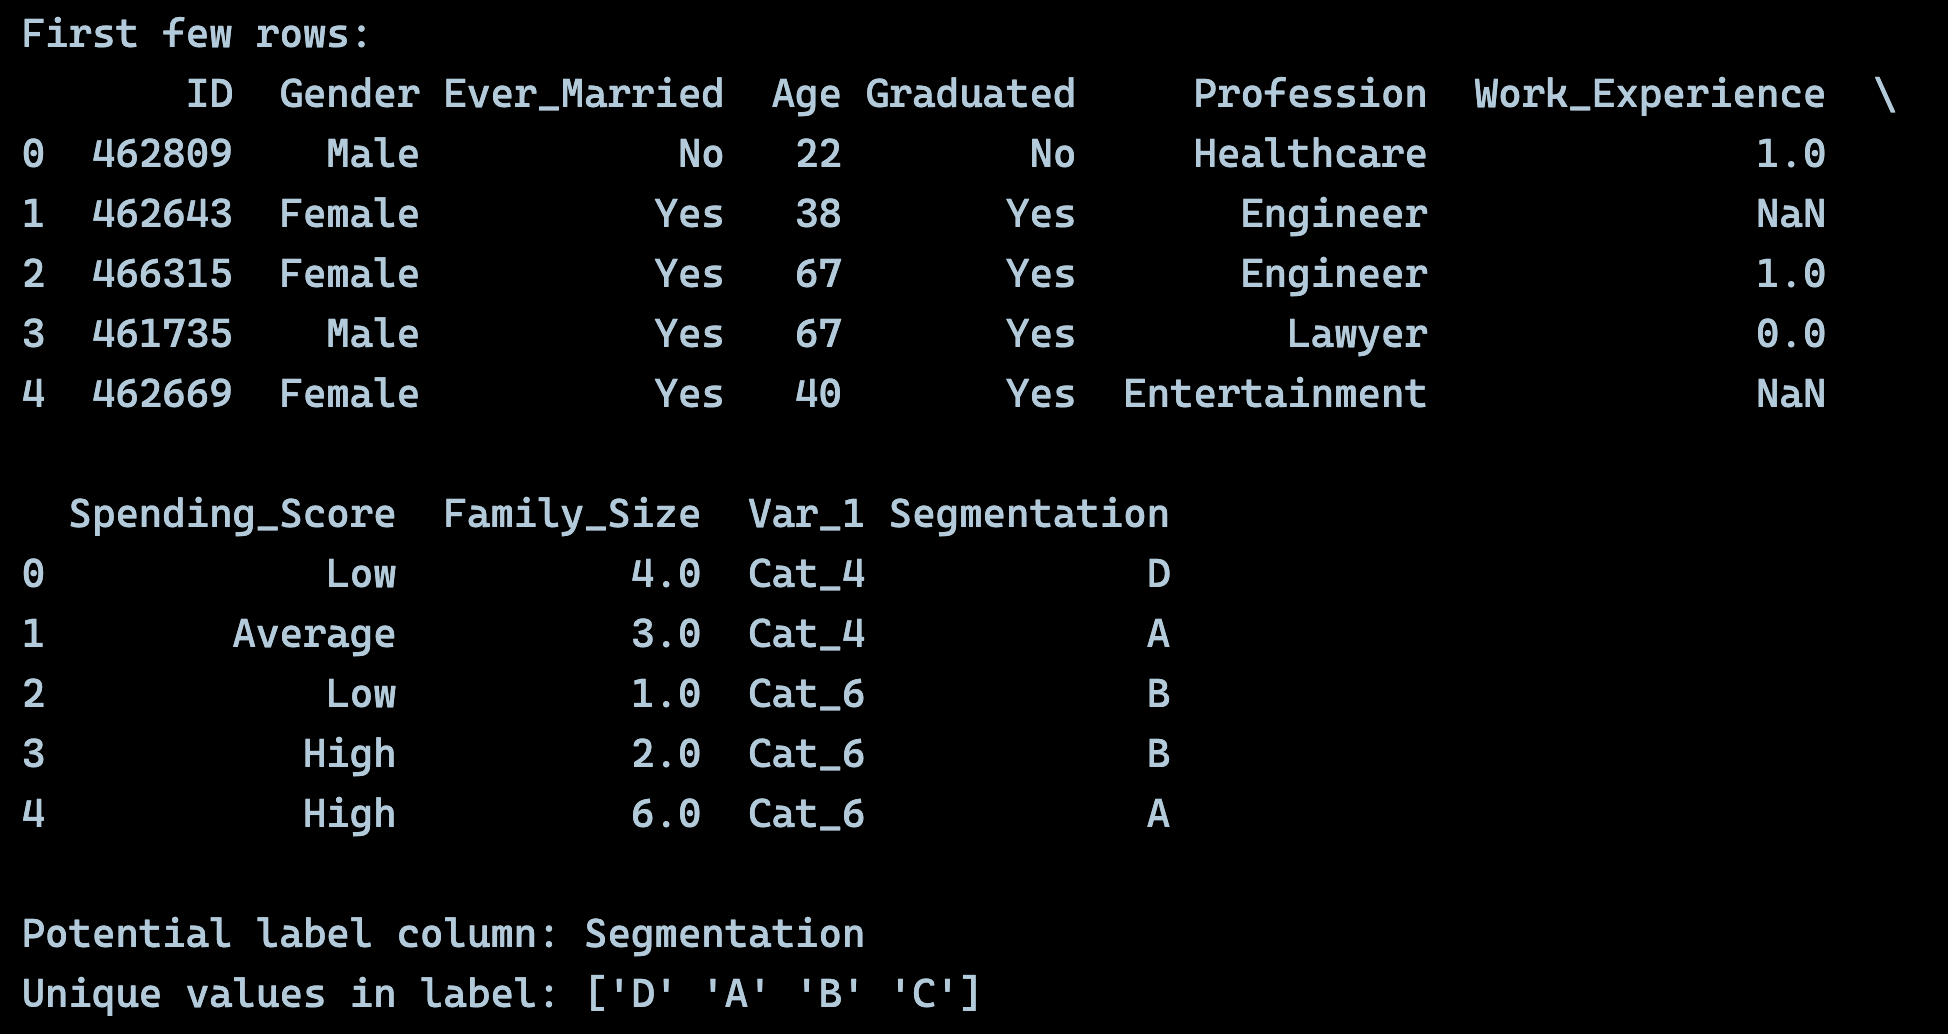
\includegraphics[width=0.70\textwidth]{Figures/label_column_info.png}
    \caption{Labeled Column Info}
\end{figure}

\subsection{Data Splitting (Training, Validation, and Test Sets)}

\subsubsection{Implementation Approach}
I split the data into three sets using train\_test\_split function twice to achieve the required 60\% training, 20\% validation, and 20\% test distribution. My technique involved a two-step splitting process: first, I separated 20\% of the data as the final test set, then I split the remaining 80\% into training (60\% of total) and validation (20\% of total) sets. I set random\_state=42 to ensure reproducible results across multiple runs. This approach gave me a proper train-validation-test setup where I could train models on the training set, tune hyperparameters using the validation set, and evaluate final performance on the unseen test set.

\subsubsection{Implementation Code}
\begin{lstlisting}[language=Python, caption={Data Splitting into Training Validation and Test Sets}]
# Splitting data into train, validation, and test sets (60-20-20)
X_temp, X_test, y_temp, y_test = train_test_split(df.drop(df.columns[-1], axis=1), df[df.columns[-1]], 
                                                  test_size=0.2, random_state=42)
X_train, X_val, y_train, y_val = train_test_split(X_temp, y_temp, test_size=0.25, random_state=42)

print(f"Training set: {len(X_train)} samples")
print(f"Validation set: {len(X_val)} samples")
print(f"Test set: {len(X_test)} samples")
\end{lstlisting}

\subsubsection{Terminal Output}
\begin{figure}[h!]
\centering
    
\includegraphics[width=\textwidth]{Figures/split_output.png}
    \caption{Data Splitting Results}
\end{figure}

\subsection{Variables Identification}

\subsubsection{Implementation Approach}
I clearly identified which variables were independent (features) and which was dependent (target) for my analysis. My approach was to systematically separate the dataset components by using column indexing. I extracted all columns except the last one as independent variables, while treating the last column as the dependent variable. I chose to store these in lists and print them to verify the separation was correct. This step was essential for organizing my data properly before building machine learning models and ensuring I understood which features would be used for prediction.

\subsubsection{Implementation Code}
\begin{lstlisting}[language=Python, caption=Dependent and Independent Variables Identification]
# Identifying dependent and independent variables
independent_vars = df.columns[:-1].tolist()
dependent_var = df.columns[-1]

print(f"Independent variables (features): {independent_vars}")
print(f"Dependent variable (target): {dependent_var}")
\end{lstlisting}

\subsubsection{Terminal Output}
\begin{figure}[h!]
\centering
    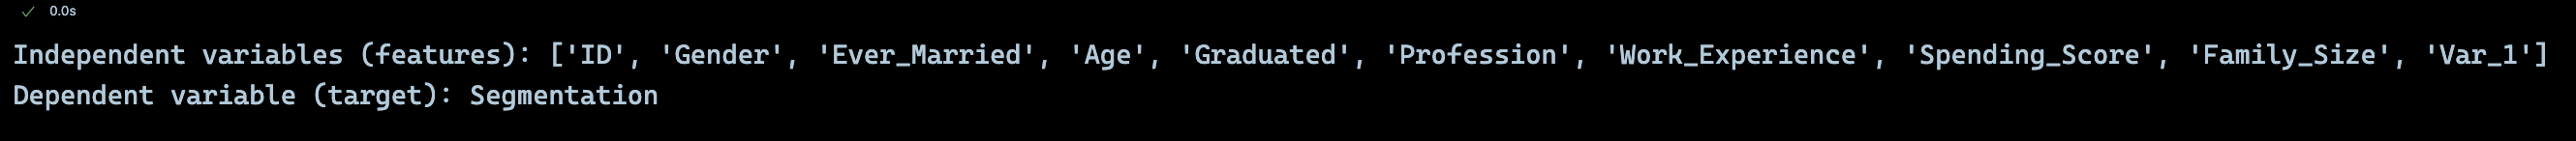
\includegraphics[width=\textwidth]{Figures/var_identification.png}
    \caption{Dependent and Independent Variables Identification}
\end{figure}

\newpage
\subsection{Features and Labels Separation}

\subsubsection{Implementation Approach}
I separated the dataset into features (X) and labels (y) for machine learning processing. My strategy involved using pandas drop() function to remove the target column from the feature matrix and selecting only the target column for the labels. I chose this approach because most machine learning algorithms expect separate X and y arrays. I printed the shapes of both arrays to verify the separation worked correctly and to understand the dimensionality of my feature space. This clean separation was crucial for feeding the data into sklearn models later in my analysis.

\subsubsection{Implementation Code}
\begin{lstlisting}[language=Python, caption=Features and Labels Separation]
# Splitting into features and labels
features = df.drop(df.columns[-1], axis=1)
labels = df[df.columns[-1]]

print(f"Features shape: {features.shape}")
print(f"Labels shape: {labels.shape}")
\end{lstlisting}

\subsubsection{Terminal Output}

\begin{figure}[h!]
\centering
    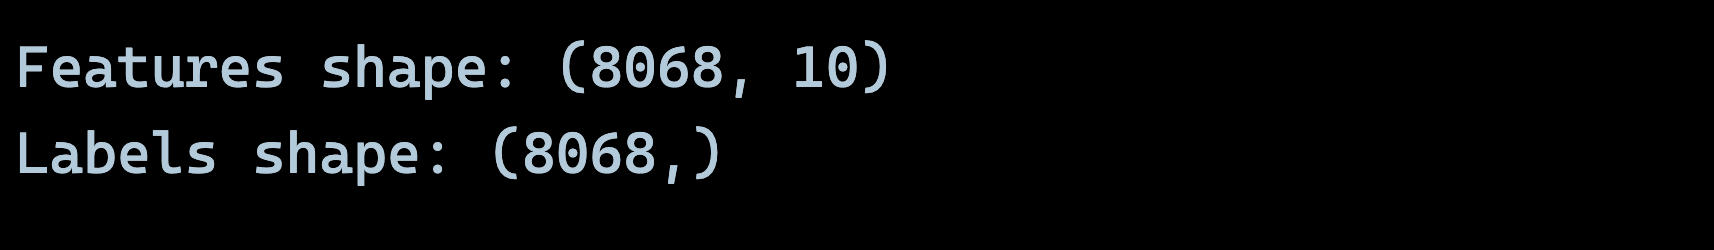
\includegraphics[width=\textwidth]{Figures/features_output.png}
    \caption{Features and Labels Separation}
\end{figure}

\subsection{Label Counts and Matplotlib Visualization}

\subsubsection{Implementation Approach}
I counted the unique labels and created a visualization to show their distribution using matplotlib. My approach involved using value\_counts() to get the frequency of each label category and nunique() to determine the total number of unique classes. I then created a bar plot visualization to make the distribution easy to understand visually. I chose matplotlib because it provides simple and effective plotting capabilities. This analysis helped me understand whether the dataset was balanced or imbalanced, which would influence my choice of evaluation metrics and modeling strategies later.

\newpage
\subsubsection{Implementation Code}
\begin{lstlisting}[language=Python, caption=Label Count Analysis and Matplotlib Visualization]
# Counting and plotting labels
num_labels = labels.nunique()
label_counts = labels.value_counts()

print(f"Number of unique labels: {num_labels}")
print(f"Label distribution:")
print(label_counts)

# Plotting label distribution
plt.figure(figsize=(8, 5))
label_counts.plot(kind='bar')
plt.title('Label Distribution')
plt.xlabel('Labels')
plt.ylabel('Count')
plt.show()
\end{lstlisting}

\subsubsection{Terminal Output}

\begin{figure}[h!]
\centering
\begin{subfigure}[b]{0.45\textwidth}
    \centering
    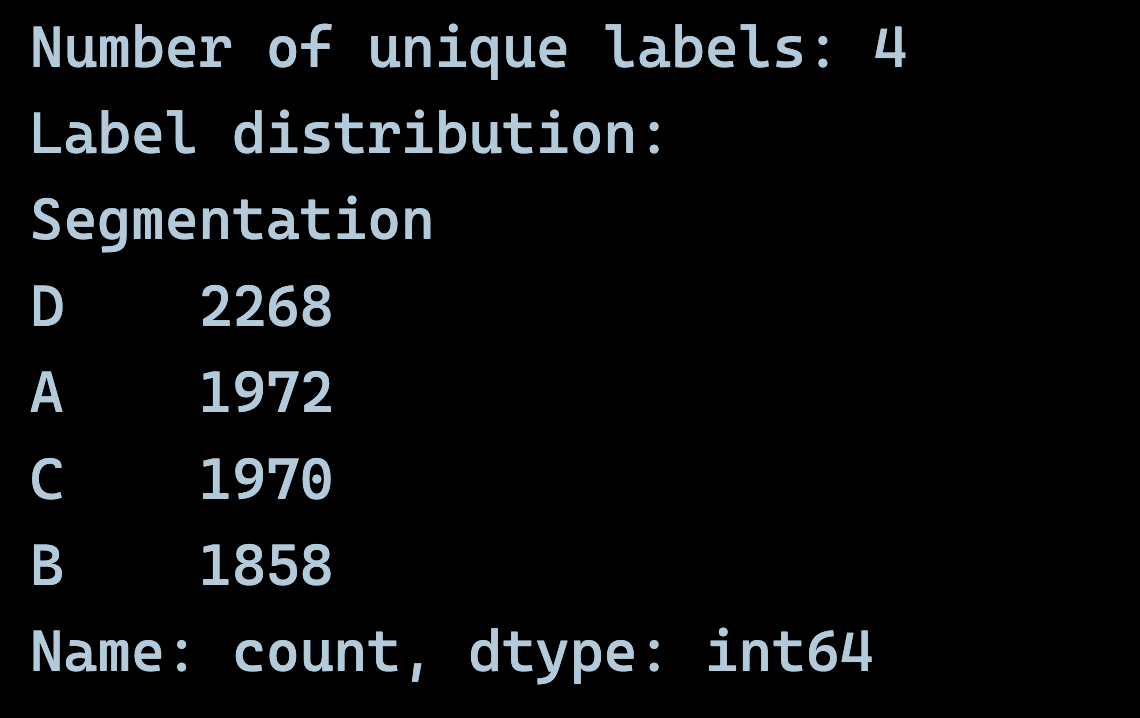
\includegraphics[width=\textwidth]{Figures/unique_labels_count.png}
    \caption{Unique Labels Count}
    \label{fig:unique_labels}
\end{subfigure}
\hfill
\begin{subfigure}[b]{0.45\textwidth}
    \centering
    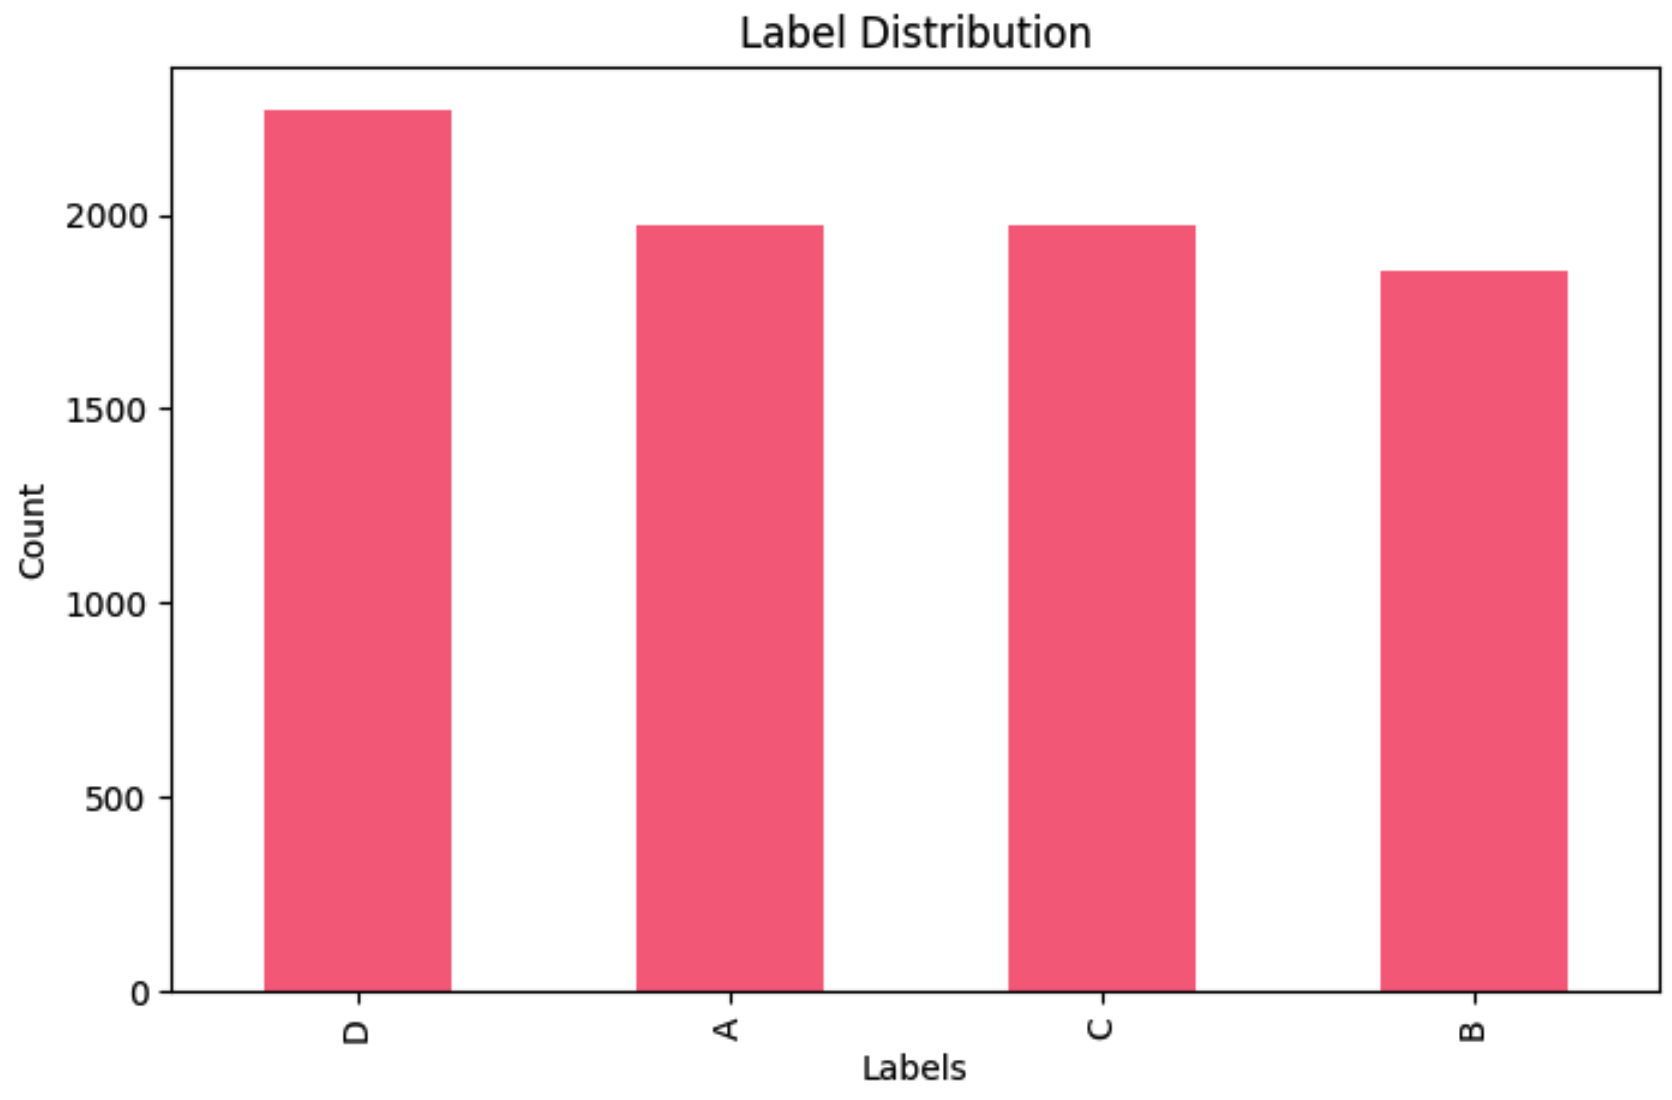
\includegraphics[width=\textwidth]{Figures/label_distribution_plot.png}
    \caption{Label Distribution Plot}
    \label{fig:label_plot}
\end{subfigure}
\caption{Label Count Analysis and Visualization Results}
\label{fig:label_analysis}
\end{figure}

\subsection{Problem Type Identification and Reasoning}

\subsubsection{Implementation Approach}
I analyzed the nature of the labels to determine what type of machine learning problem this represented (classification, multiclass classification, regression, or clustering). My approach involved checking the data type of the target variable and counting unique values to classify the problem type. I used conditional logic to determine if the labels were categorical (object or category dtype) and then counted unique values to distinguish between binary and multiclass classification. If the data type was numerical, I would classify it as a regression problem. This systematic approach helped me understand what algorithms and evaluation metrics would be appropriate for this specific problem.

\subsubsection{Implementation Code}
\begin{lstlisting}[language=Python, caption=Problem Type Identification and Reasoning]
# Determining problem type
if labels.dtype in ['object', 'category']:
    if num_labels == 2:
        problem_type = "Binary Classification"
    elif num_labels > 2:
        problem_type = "Multiclass Classification"
else:
    problem_type = "Regression"

print(f"Problem Type: {problem_type}")
print(f"Reason: {num_labels} distinct categories in target variable")
\end{lstlisting}

\subsubsection{Terminal Output}

\begin{figure}[h!]
\centering
    
\includegraphics[width=\textwidth]{Figures/problem_type_output.png}
    \caption{Problem Type Identification and Reasoning}
\end{figure}

% ===================== MODULE 2: DATA PREPROCESSING =====================
\section{Data Pre-processing}

\subsection{Load Dataset and Handle Missing Values}

\subsubsection{Implementation Approach}
I loaded the Customer Segmentation Classification dataset and identified missing values, then applied appropriate imputation strategies to handle them effectively for further analysis. My strategy involved using different imputation techniques for different data types. I chose median imputation for numerical columns because it's robust to outliers, and mode (most frequent) imputation for categorical columns because it preserves the distribution. I first checked for missing values using isnull().sum() to understand the extent of the problem, then separated columns by data type using select\_dtypes(). I created separate SimpleImputer objects for numerical and categorical data, applying them conditionally based on whether columns of each type existed in the dataset.

\subsubsection{Implementation Code}
\begin{lstlisting}[language=Python, caption=Handle Missing Values]
from sklearn.impute import SimpleImputer
from sklearn.preprocessing import LabelEncoder, MinMaxScaler, StandardScaler

# Checking for missing values
missing_summary = df.isnull().sum()
print("Missing values per column:")
print(missing_summary[missing_summary > 0])

# Handling missing values
num_imputer = SimpleImputer(strategy='median')
cat_imputer = SimpleImputer(strategy='most_frequent')

# Creating clean copy
df_clean = df.copy()
numeric_cols = df_clean.select_dtypes(include=[np.number]).columns
categorical_cols = df_clean.select_dtypes(include=['object']).columns

# Applying imputation
if len(numeric_cols) > 0:
    df_clean[numeric_cols] = num_imputer.fit_transform(df_clean[numeric_cols])
if len(categorical_cols) > 0:
    df_clean[categorical_cols] = cat_imputer.fit_transform(df_clean[categorical_cols])

print(f"Dataset cleaned. After imputation: ")
print(f"{df_clean.isnull().sum()}")
\end{lstlisting}

\subsubsection{Terminal Output}

\begin{figure}[h!]
    \centering
    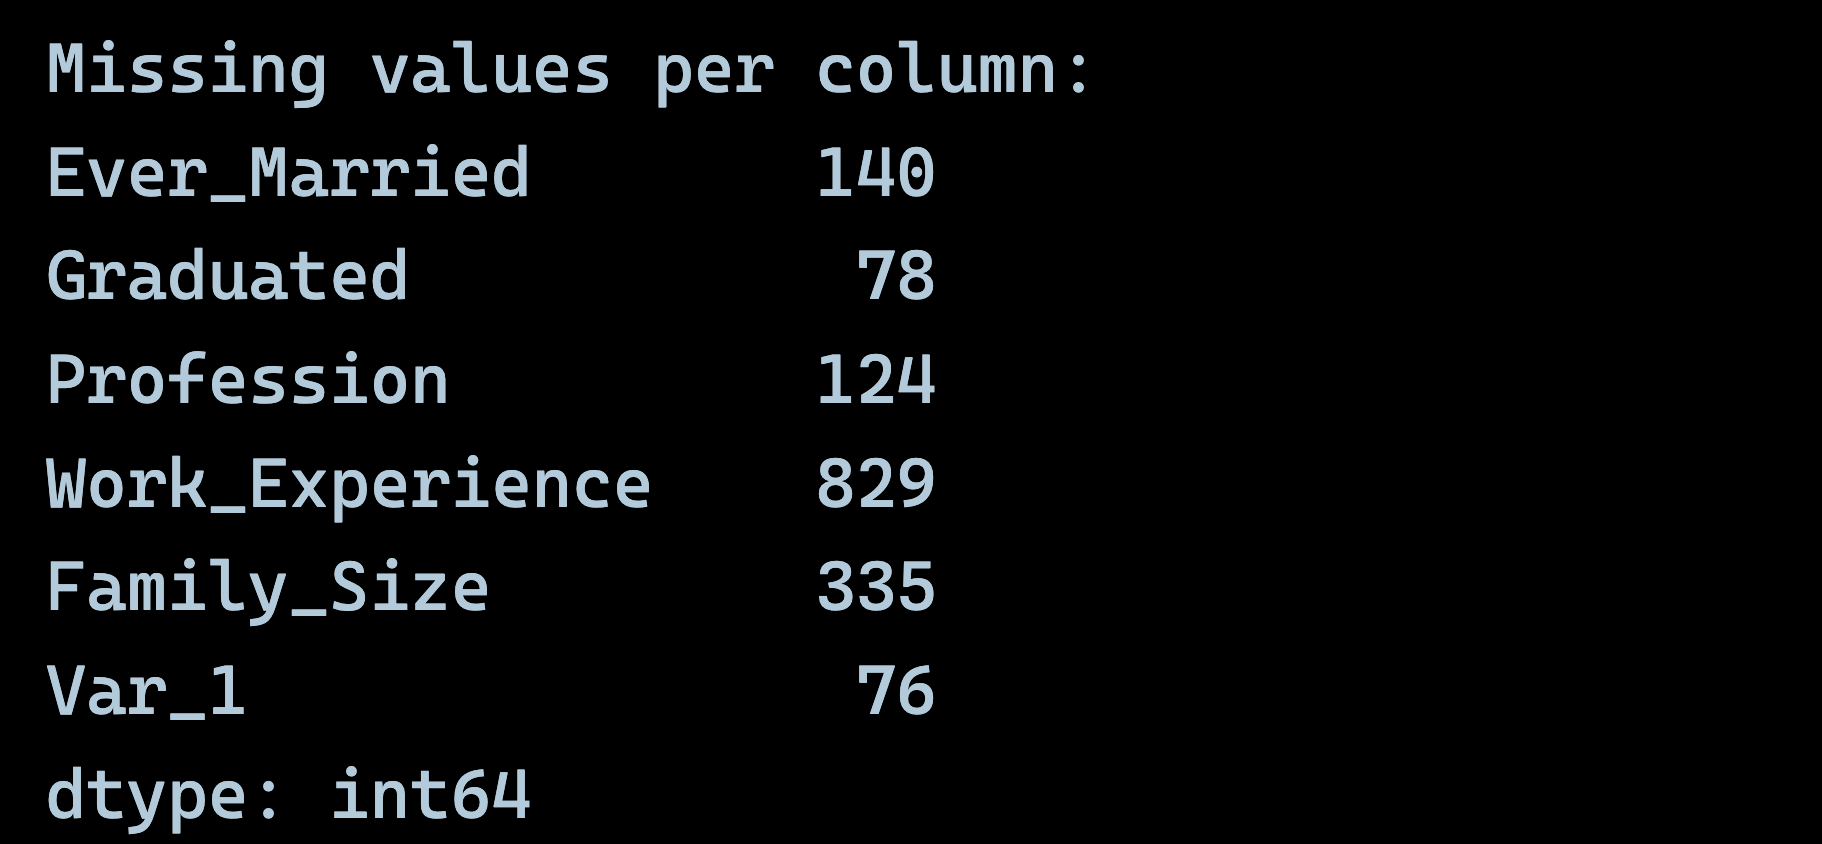
\includegraphics[width=\textwidth]{Figures/missing_values_before.png}
    \caption{Missing Values Before}
    \label{fig:missing_before}
\end{figure}

\begin{figure}[h!]
    \centering
    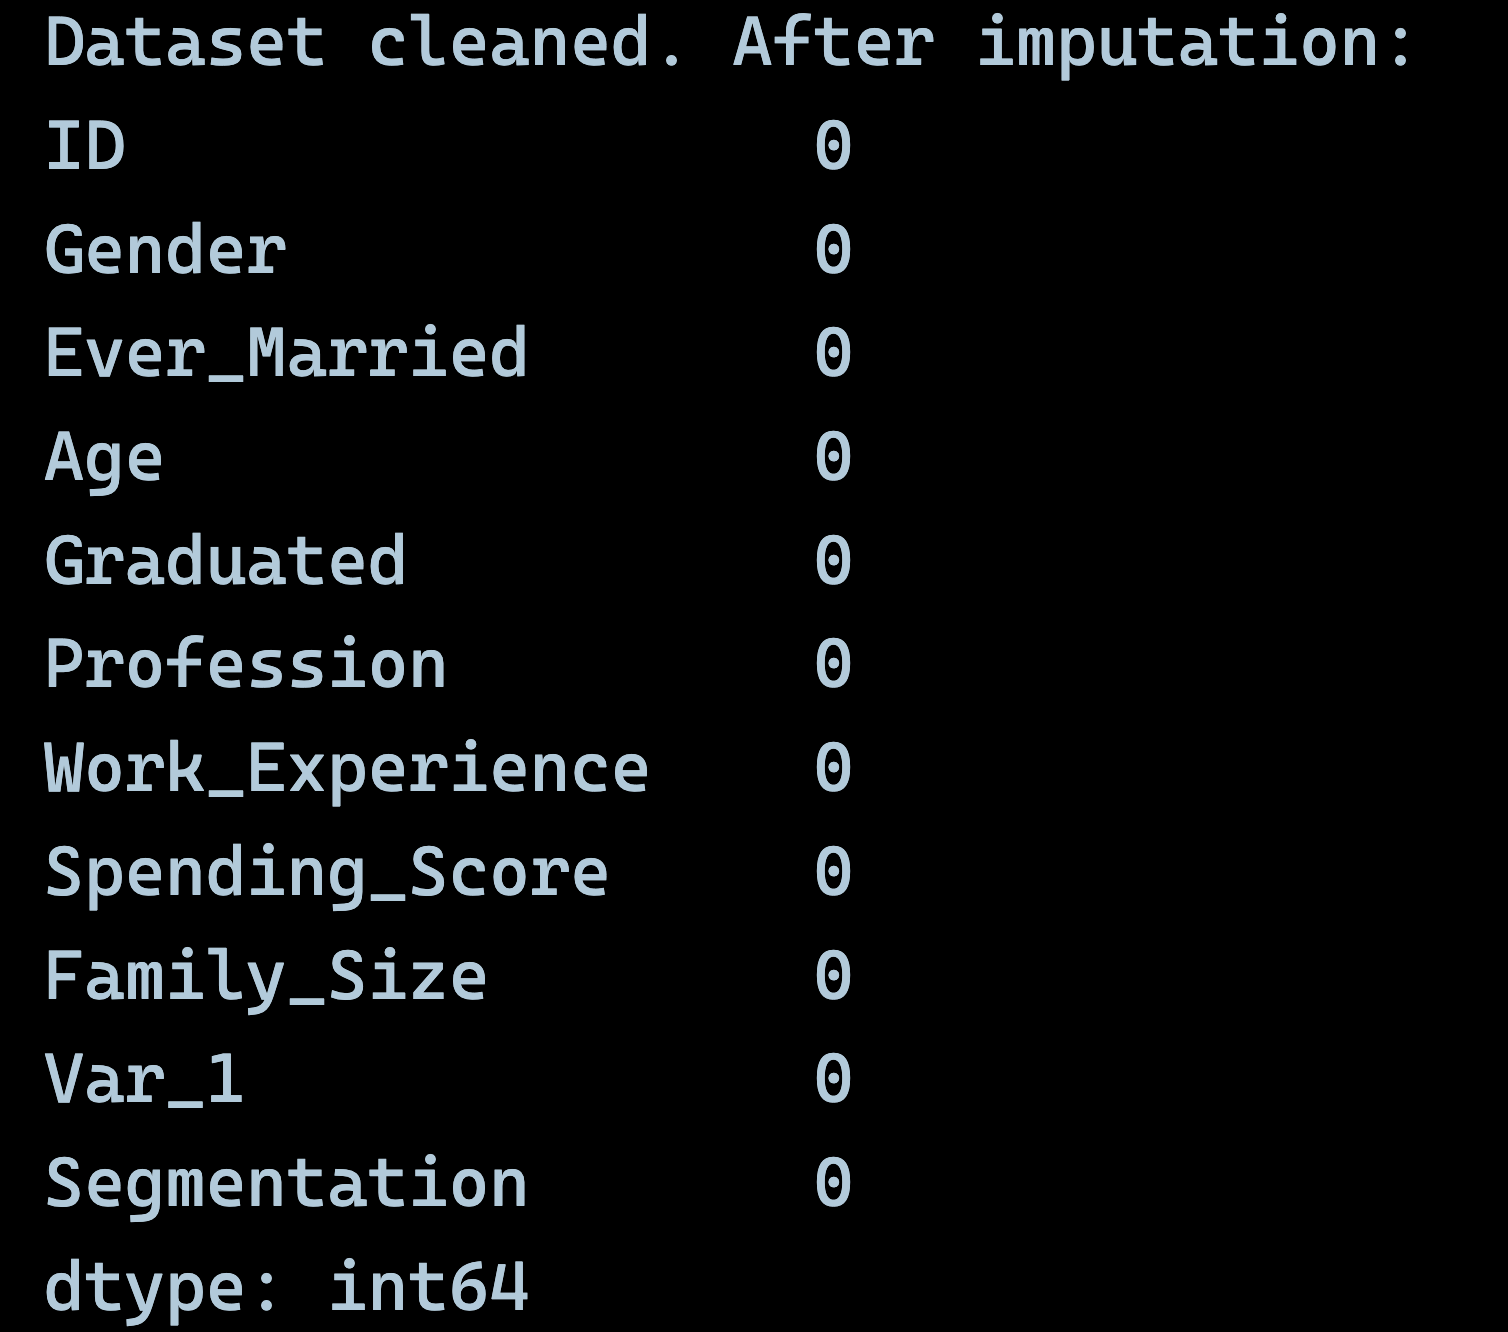
\includegraphics[width=0.6\textwidth]{Figures/missing_values_after.png}
    \caption{After Imputation Process}
    \label{fig:missing_after}
\end{figure}

\newpage
\subsection{Categorical Data Encoding}

\subsubsection{Implementation Approach}
I applied label encoding and one-hot encoding techniques to convert categorical variables into numerical format suitable for machine learning algorithms. My approach involved implementing both encoding methods to understand their differences. For label encoding, I used LabelEncoder from sklearn and stored each encoder in a dictionary to keep track of the mappings. I chose to print the mappings to understand how categories were converted to numbers. For one-hot encoding, I used pandas get\_dummies() function on one example column to demonstrate the technique. I selected label encoding as my primary method because it's more memory efficient than one-hot encoding, though I recognized that one-hot encoding might be better for non-ordinal categorical variables.

\subsubsection{Implementation Code}
\begin{lstlisting}[language=Python, caption=Categorical Data Encoding - Label Encoding and One-Hot Encoding]
# Label Encoding
df_encoded = df_clean.copy()
label_encoders = {}

# Applying label encoding
for col in categorical_cols:
    if col in df_encoded.columns:
        le = LabelEncoder()
        df_encoded[col] = le.fit_transform(df_encoded[col])
        label_encoders[col] = le

print("Encoded columns with mappings:")
for col, encoder in label_encoders.items():
    mapping = dict(zip(encoder.classes_, range(len(encoder.classes_))))
    print(f"  {col}: {mapping}")

# One-hot encoding
if len(categorical_cols) > 0:
    example_col = categorical_cols[0]
    df_onehot = pd.get_dummies(df_clean, columns=[example_col], prefix=example_col)
    print(f"\nOne-hot encoding applied to: {example_col}")
    print(f"Shape change: {df_clean.shape} -> {df_onehot.shape}")
else:
    df_onehot = df_clean.copy()
\end{lstlisting}

\subsubsection{Terminal Output}

\begin{figure}[h!]
\centering
    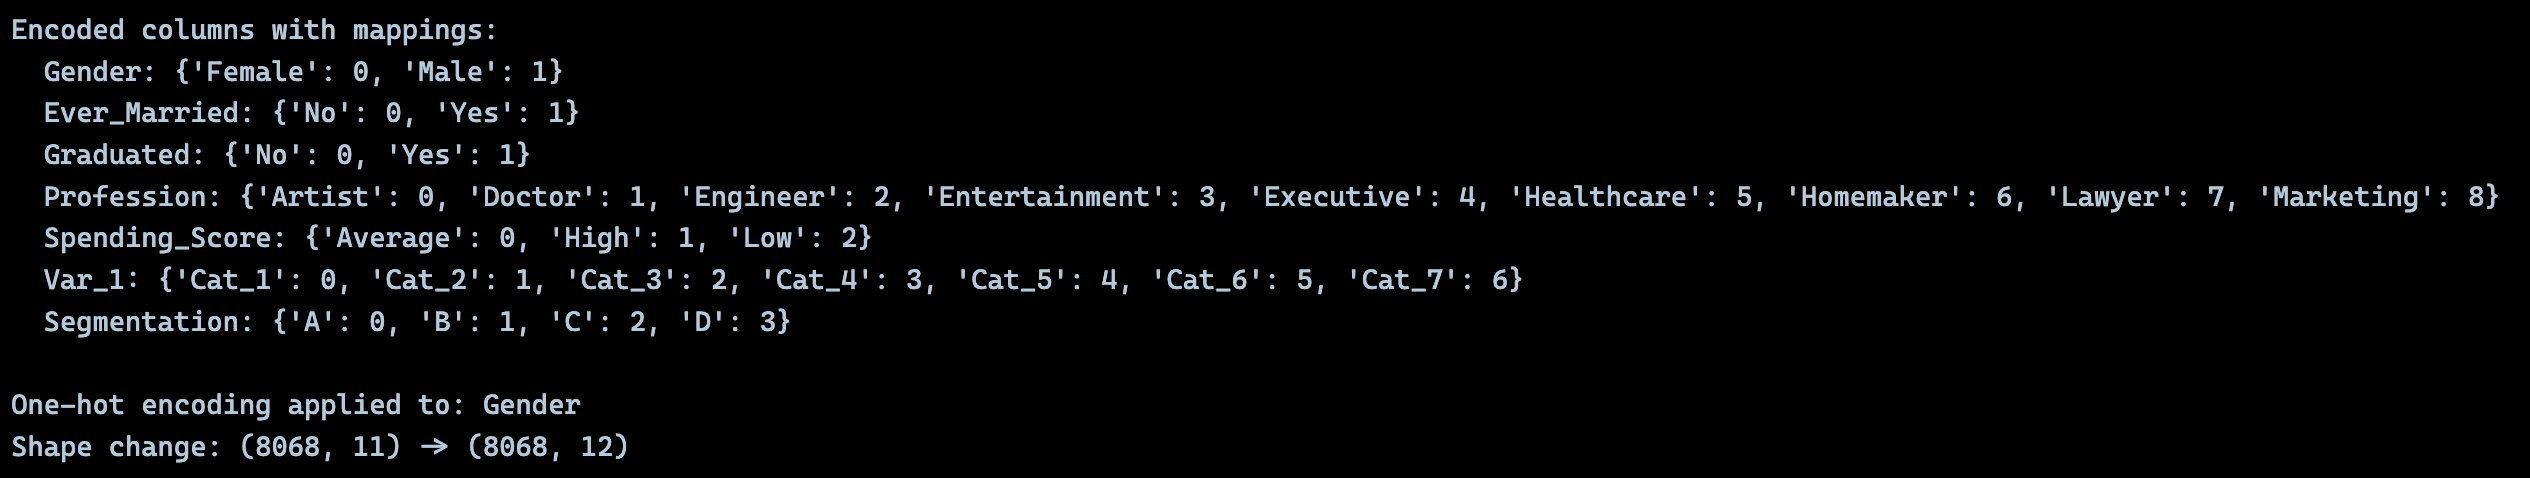
\includegraphics[width=\textwidth]{Figures/encoding_output.png}
    \caption{Categorical Data Encoding - Label Encoding and One-Hot Encoding}
\end{figure}

\subsection{Feature Scaling Methods}

\subsubsection{Implementation Approach}
I performed feature scaling using both min-max normalization and z-score standardization to ensure all numerical features were on the same scale. My strategy was to implement these scaling methods manually to understand the underlying mathematics. I chose to create custom functions rather than using sklearn's built-in scalers to demonstrate the mathematical concepts. For min-max normalization, I implemented the formula (x - min) / (max - min) to scale values between 0 and 1. For z-score standardization, I calculated (x - mean) / standard\_deviation to center data around zero with unit variance. I applied these techniques to selected numerical features and compared the results to understand how different scaling methods affect the data distribution.

\subsubsection{Implementation Code}
\begin{lstlisting}[language=Python, caption=Feature Scaling - Min-Max Normalization and Z-Score Standardization]
import math
def min_max_normalize_manual(data):
    normalized_data = data.copy().astype(float)
    
    for column in data.columns:
        col_min = data[column].min()
        col_max = data[column].max()
        
        for i in data.index:
            original_val = data.loc[i, column]
            normalized_val = (original_val - col_min) / (col_max - col_min)
            normalized_data.loc[i, column] = normalized_val
    return normalized_data

def z_score_standardize_manual(data):
    standardized_data = data.copy().astype(float)
    for column in data.columns:
        col_mean = sum(data[column]) / len(data[column])
        squared_diffs = [(x - col_mean) ** 2 for x in data[column]]
        variance = sum(squared_diffs) / (len(data[column]) - 1)
        col_std = math.sqrt(variance)
    
        for i in data.index:
            original_val = data.loc[i, column]
            standardized_val = (original_val - col_mean) / col_std
            standardized_data.loc[i, column] = standardized_val
    return standardized_data

# Applying scaling to selected features
selected_features = ['Age', 'Work_Experience', 'Family_Size'] 
sample_data = df_clean[selected_features].head(100)
minmax_normalized = min_max_normalize_manual(sample_data)
zscore_standardized = z_score_standardize_manual(sample_data)

# Displaying results
print("Selected features:", selected_features)
print("\nMin-Max Normalized (first 5 samples):")
print(minmax_normalized.head(5))
print("\nZ-Score Standardized (first 5 samples):")
print(zscore_standardized.head(5))
\end{lstlisting}

\subsubsection{Terminal Output}

\begin{figure}[h!]
\centering
    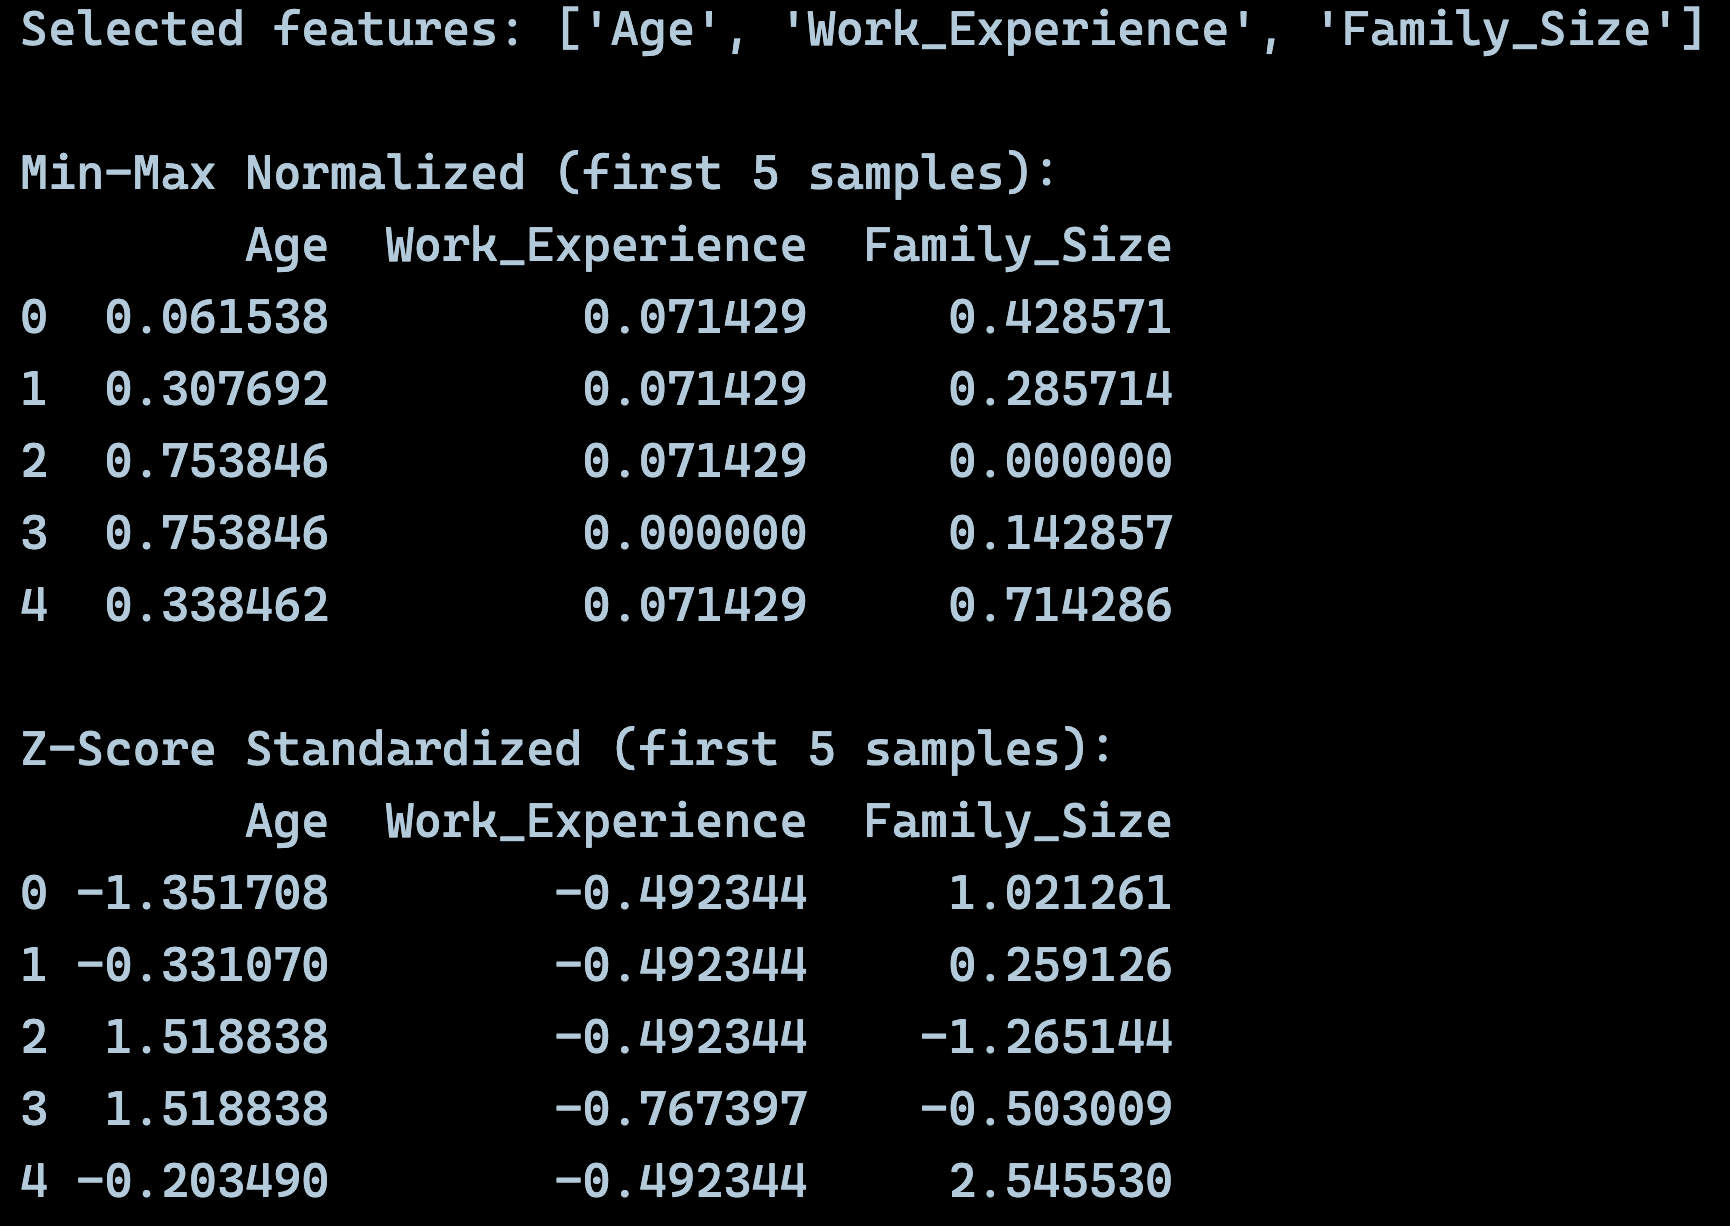
\includegraphics[width=0.5\textwidth]{Figures/scaling_output.png}
    \caption{Feature Scaling - Min-Max Normalization and Z-Score Standardization}
\end{figure}

\subsection{Similarity and Dissimilarity Measures}

\subsubsection{Implementation Approach}
I implemented four different similarity and distance measures using manual calculations without library functions: Pearson's Correlation, Cosine Similarity, Jaccard Similarity, and Euclidean Distance to analyze relationships between data points with step-by-step mathematical formulations. My approach was to code each measure from scratch to understand the mathematical foundations. I chose Pearson correlation to measure linear relationships, cosine similarity for directional similarity, Jaccard similarity for binary relationships (after converting data to binary), and Euclidean distance for geometric proximity. I implemented each function manually by calculating means, standard deviations, and other statistical measures step by step. I then applied these measures to normalized data vectors to compare different customer profiles and understand their relationships.

\subsubsection{Implementation Code}
\begin{lstlisting}[language=Python, caption=Manual Similarity and Dissimilarity Measures]
def pearson_correlation_manual(x, y):
    n = len(x)
    x_mean = sum(x) / n
    y_mean = sum(y) / n
    
    numerator = sum((x[i] - x_mean) * (y[i] - y_mean) for i in range(n))
    sum_x_sq = sum((x[i] - x_mean) ** 2 for i in range(n))
    sum_y_sq = sum((y[i] - y_mean) ** 2 for i in range(n))
    
    denominator = math.sqrt(sum_x_sq * sum_y_sq)
    return numerator / denominator if denominator != 0 else 0

def cosine_similarity_manual(x, y):
    dot_product = sum(x[i] * y[i] for i in range(len(x)))
    magnitude_x = math.sqrt(sum(x[i] ** 2 for i in range(len(x))))
    magnitude_y = math.sqrt(sum(y[i] ** 2 for i in range(len(y))))
    
    return dot_product / (magnitude_x * magnitude_y) if magnitude_x != 0 and magnitude_y != 0 else 0

def jaccard_similarity_manual(x, y):
    # Converting to binary (1 if above median, 0 otherwise)
    median_x = sorted(x)[len(x)//2]
    median_y = sorted(y)[len(y)//2]
    
    binary_x = [1 if val > median_x else 0 for val in x]
    binary_y = [1 if val > median_y else 0 for val in y]
    
    # Calculate intersection and union manually
    intersection = sum(1 for i in range(len(binary_x)) if binary_x[i] == 1 and binary_y[i] == 1)
    union = sum(1 for i in range(len(binary_x)) if binary_x[i] == 1 or binary_y[i] == 1)
    
    return intersection / union if union != 0 else 0

def euclidean_distance_manual(x, y):
    """Manual implementation of Euclidean distance"""
    sum_squared_diff = sum((x[i] - y[i]) ** 2 for i in range(len(x)))
    return math.sqrt(sum_squared_diff)

# Creating sample vectors and calculating similarities
vectors = []
for i in range(3):
    vector = minmax_normalized.iloc[i].values
    vectors.append(vector)

# Calculating all pairwise similarities
for i in range(len(vectors)):
    for j in range(i+1, len(vectors)):
        pearson_corr = pearson_correlation_manual(vectors[i], vectors[j])
        cosine_sim = cosine_similarity_manual(vectors[i], vectors[j])
        jaccard_sim = jaccard_similarity_manual(vectors[i], vectors[j])
        euclidean_dist = euclidean_distance_manual(vectors[i], vectors[j])
        
        print(f"Vector {i+1} vs Vector {j+1}:")
        print(f"  Pearson Correlation: {pearson_corr:.4f}")
        print(f"  Cosine Similarity: {cosine_sim:.4f}")
        print(f"  Jaccard Similarity: {jaccard_sim:.4f}")
        print(f"  Euclidean Distance: {euclidean_dist:.4f}")
\end{lstlisting}

\subsubsection{Terminal Output}

\begin{figure}[h!]
\centering
    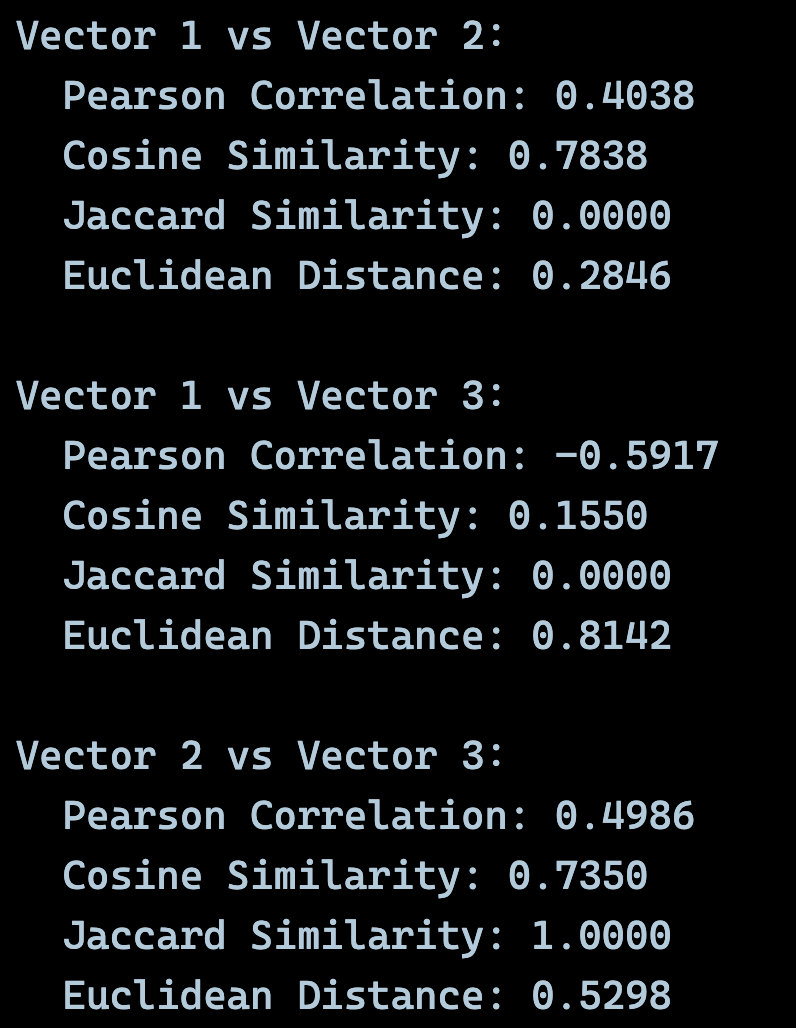
\includegraphics[width=0.4\textwidth]{Figures/similarity_output.png}
    \caption{Similarity and Dissimilarity Measures Results}
\end{figure}


\newpage
% ===================== MODULE 3: EXPLORATORY DATA ANALYSIS =====================
\section{Exploratory Data Analysis}

\subsection{Plot Distributions of Variables}

\subsubsection{Implementation Approach}
I plotted the distributions of both numerical and categorical variables to understand the data patterns and identify the shape of the distributions. My strategy involved creating separate visualizations for different data types. For numerical variables, I used histograms with 20 bins to show the frequency distribution and identify patterns like skewness or normality. I chose specific variables like Age, Work\_Experience, and Family\_Size as representative numerical features. For categorical variables, I used bar plots showing value counts to understand the frequency of each category. I applied consistent styling with colors, transparency, and grid lines to make the plots professional and easy to interpret. This exploratory analysis helped me understand the data distribution before applying any transformations.

\subsubsection{Implementation Code}
\begin{lstlisting}[language=Python, caption=Plot Distributions of Variables]
# Plotting distributions for specific numerical variables 
numerical_cols = ['Age', 'Work_Experience', 'Family_Size']

plt.figure(figsize=(12, 4))
for i, col in enumerate(numerical_cols):
    plt.subplot(1, 3, i+1)
    plt.hist(df_clean[col], bins=20, alpha=0.7, color='skyblue', edgecolor='black')
    plt.title(f'Distribution of {col}')
    plt.xlabel(col)
    plt.ylabel('Frequency')
    plt.grid(True, alpha=0.3)

plt.tight_layout()
plt.show()

# Plotting distributions for specific categorical variables
categorical_cols = ['Gender', 'Graduated', 'Profession', 'Ever_Married', 'Var_1', 'Segmentation']

plt.figure(figsize=(15, 8))
for i, col in enumerate(categorical_cols):
    plt.subplot(2, 3, i+1)
    df_clean[col].value_counts().plot(kind='bar', color='lightcoral', alpha=0.8)
    plt.title(f'Distribution of {col}')
    plt.xlabel(col)
    plt.ylabel('Count')
    plt.xticks(rotation=45)
    plt.grid(True, alpha=0.3)
plt.tight_layout()
plt.show()
\end{lstlisting}

\subsubsection{Terminal Output}

\begin{figure}[h!]
\centering
\begin{subfigure}[b]{\textwidth}
    \centering
    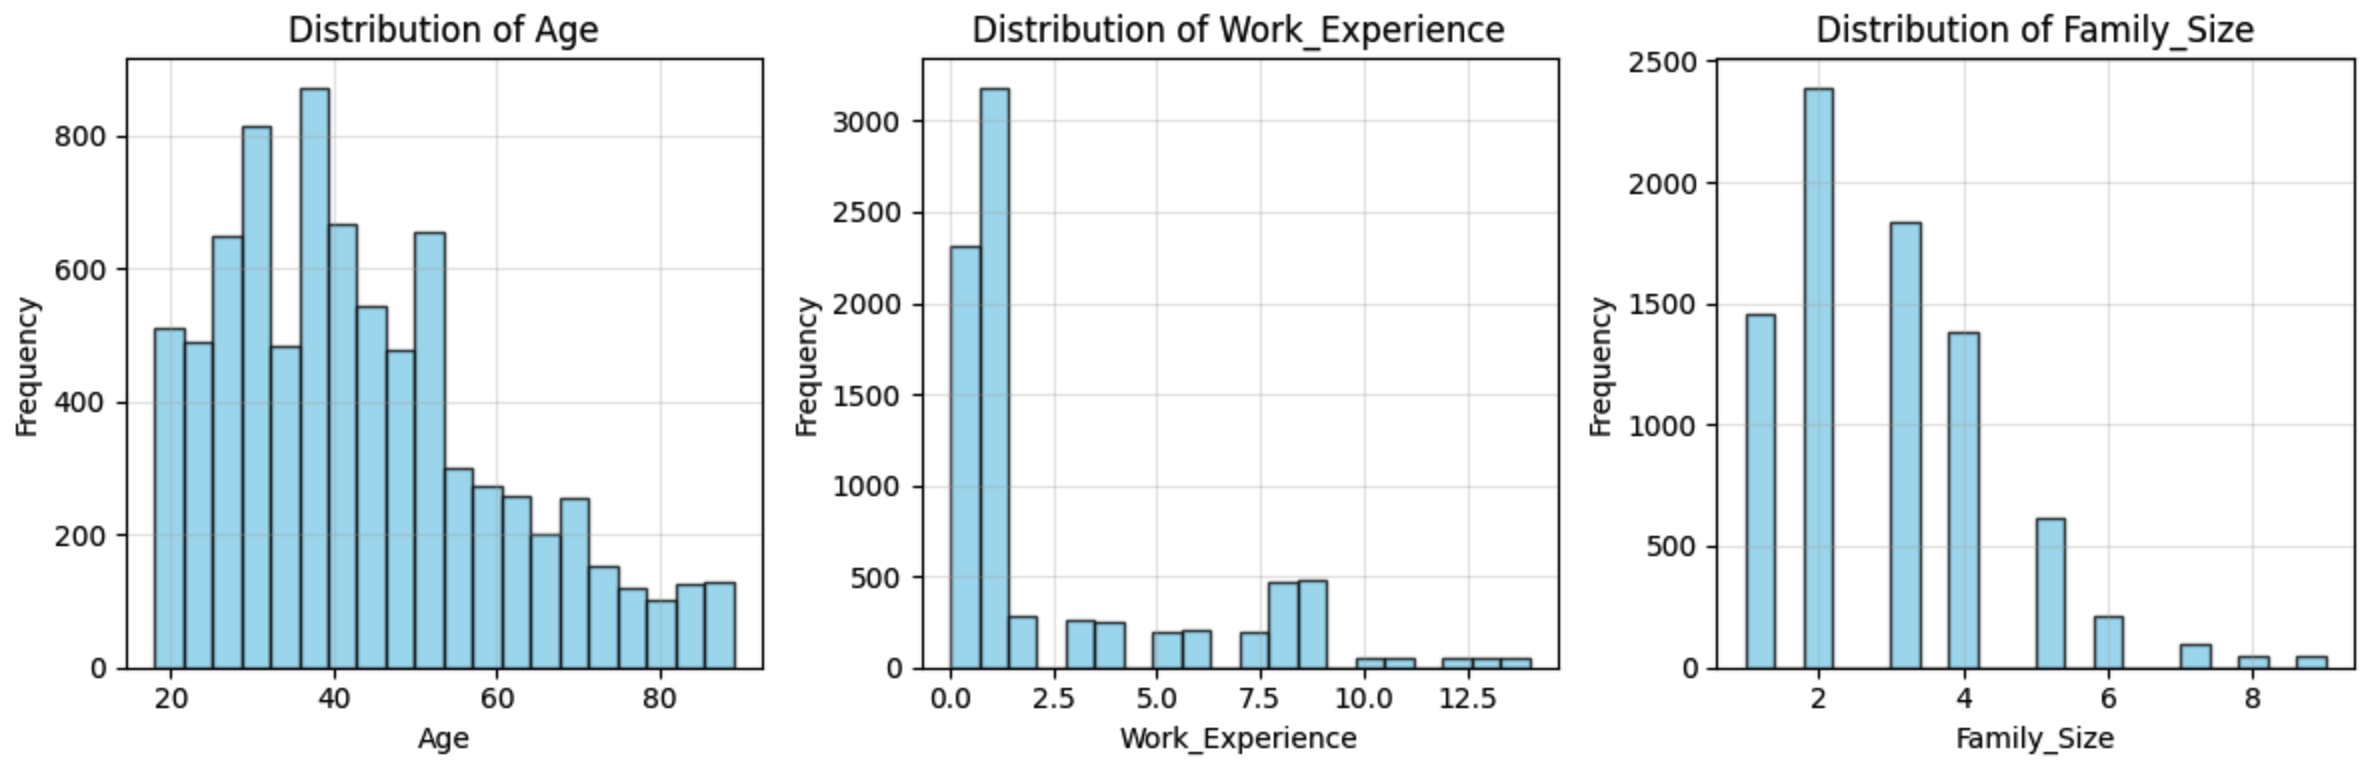
\includegraphics[width=\textwidth]{Figures/numerical_distributions.png}
    \caption{Numerical Variables Distribution}
    \label{fig:numerical_dist}
\end{subfigure}
\hfill

\begin{subfigure}[b]{\textwidth}
    \centering
    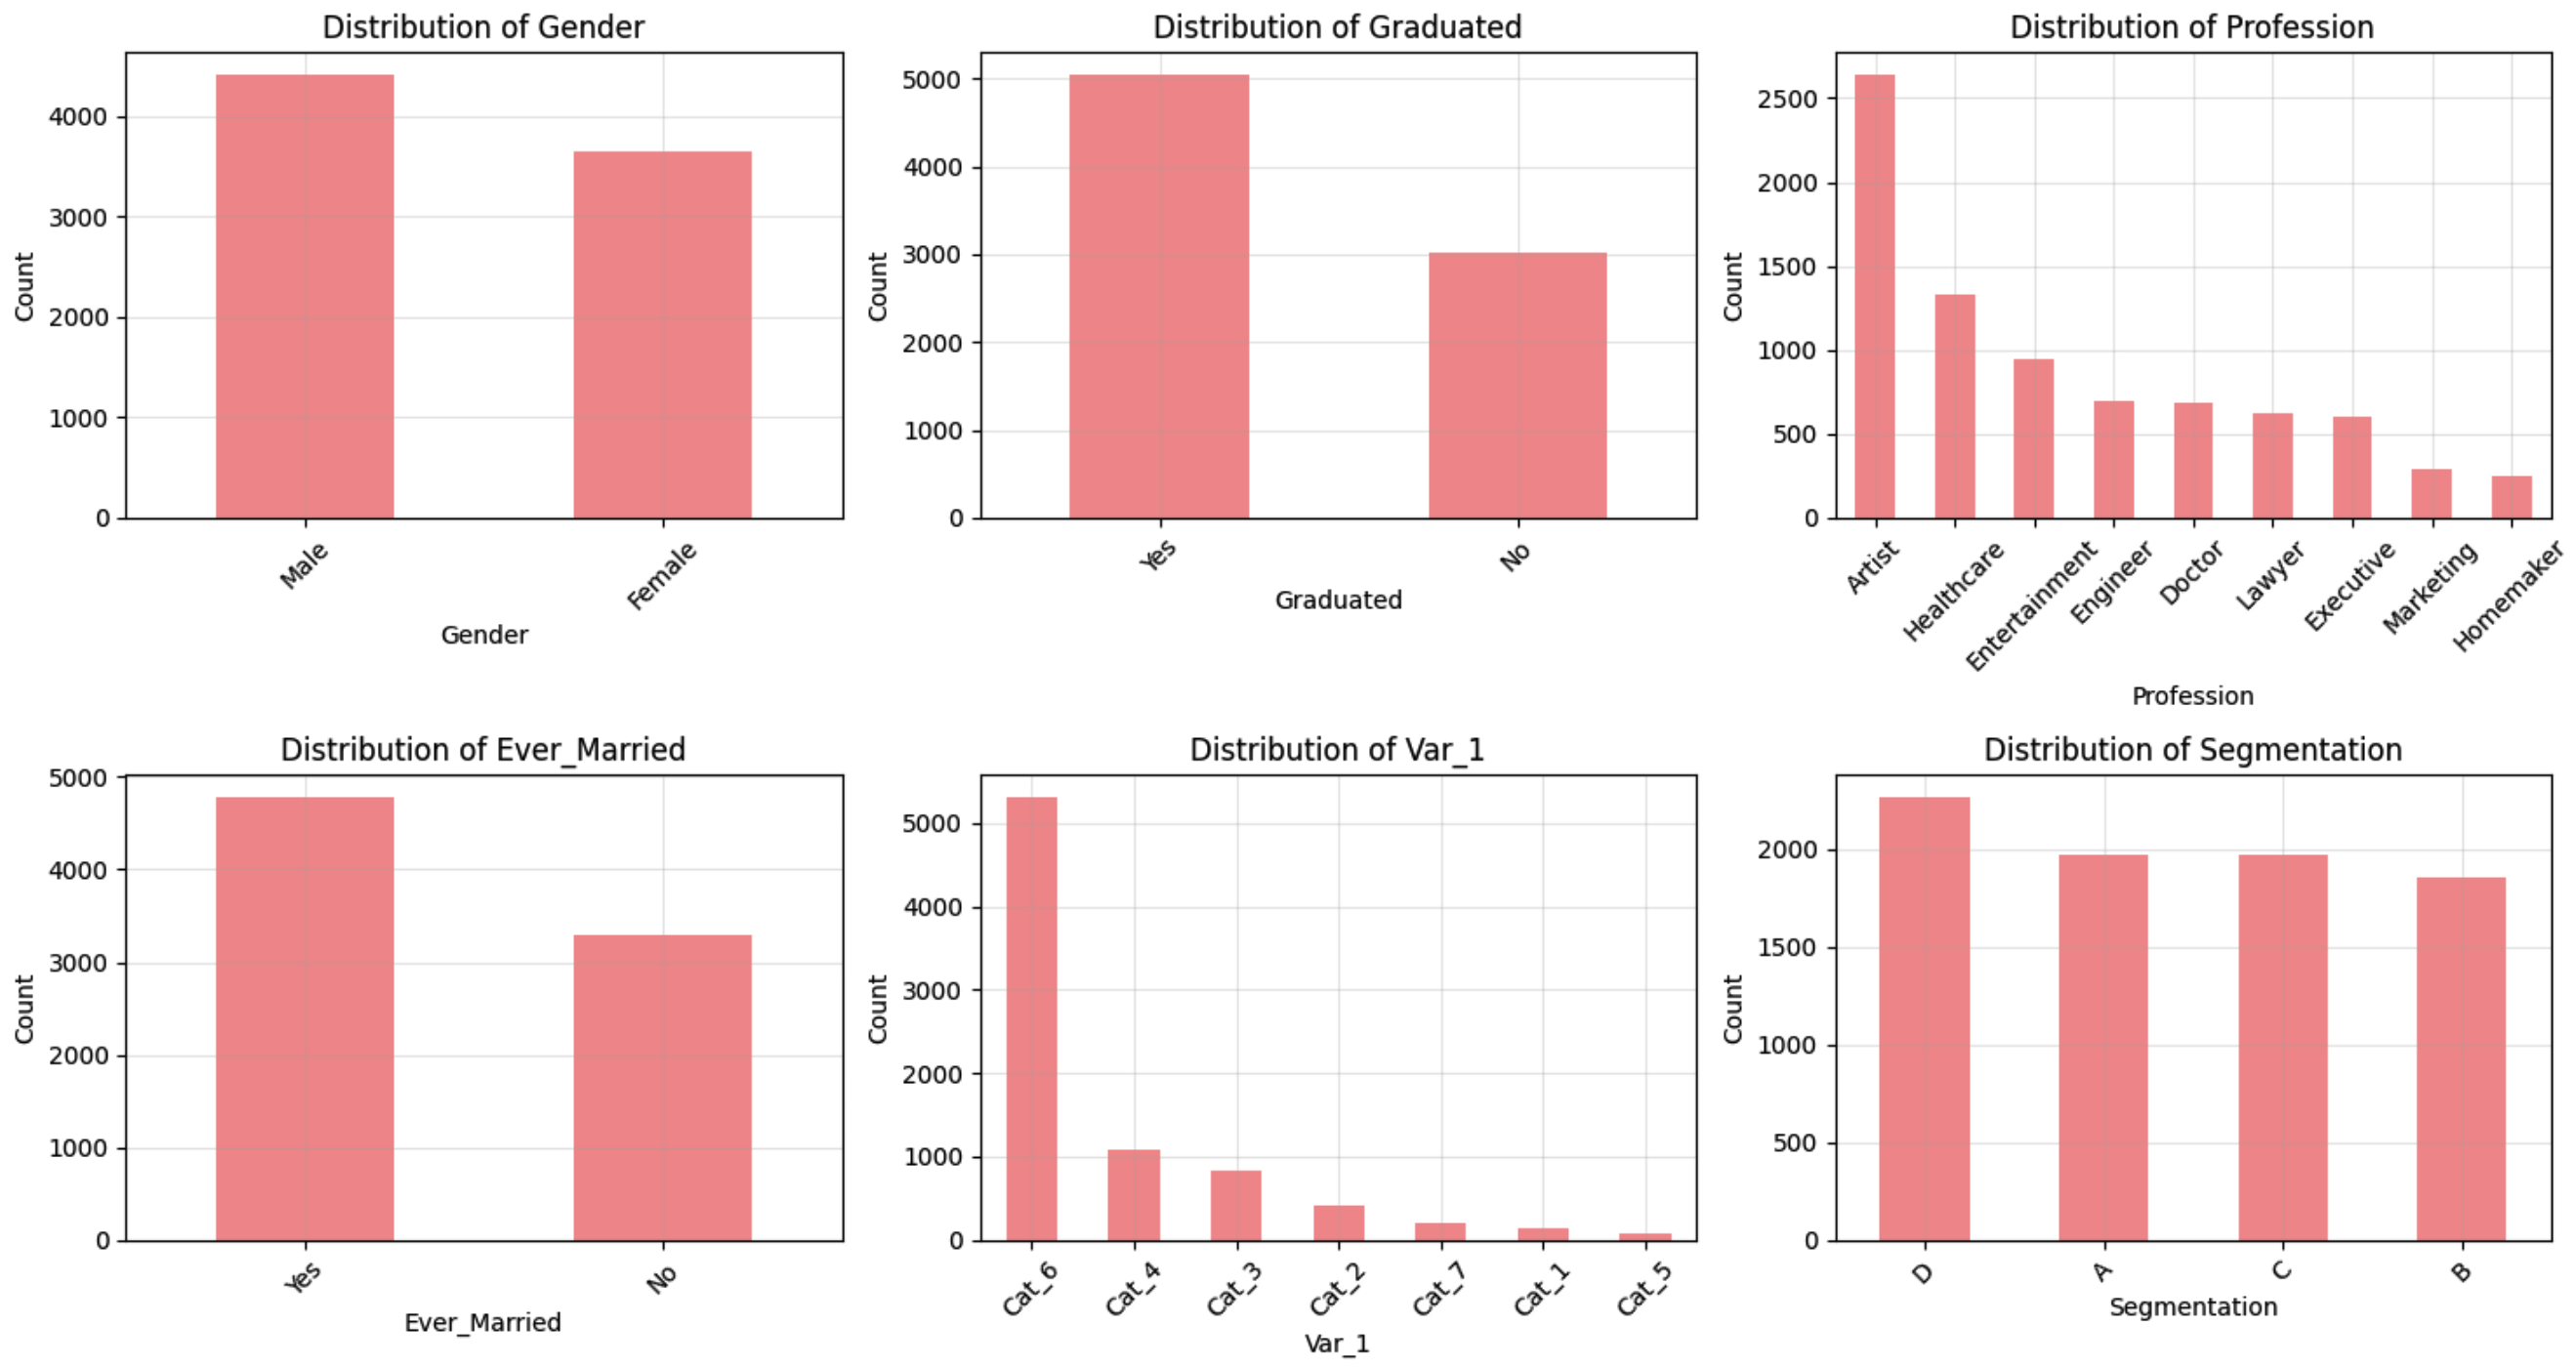
\includegraphics[width=\textwidth]{Figures/categorical_distributions.png}
    \caption{Categorical Variables Distribution}
    \label{fig:categorical_dist}
\end{subfigure}
\caption{Distributions of Numerical and Categorical Variables}
\label{fig:variable_distributions}
\end{figure}

\subsection{Identify Outliers Using Boxplots}

\subsubsection{Implementation Approach}
I created boxplots for numerical variables to identify outliers and understand the spread of the data. My approach involved using matplotlib's boxplot function to visualize the five-number summary (minimum, Q1, median, Q3, maximum) and identify outliers as points beyond the whiskers. I implemented a systematic outlier detection method using the IQR (Interquartile Range) technique, calculating Q1, Q3, and IQR, then defining outliers as values below Q1-1.5*IQR or above Q3+1.5*IQR. I chose this method because it's a standard statistical approach for outlier detection. 

\subsubsection{Implementation Code}
\begin{lstlisting}[language=Python, caption=Identify Outliers Using Boxplots]
# Creating boxplots to identify outliers
plt.figure(figsize=(12, 8))
for i, col in enumerate(numerical_cols):
    plt.subplot(2, 3, i+1)
    plt.boxplot(df_clean[col])
    plt.title(f'Boxplot of {col}')
    plt.ylabel(col)

plt.tight_layout()
plt.show()

# Printing outlier information
for col in numerical_cols:
    Q1 = df_clean[col].quantile(0.25)
    Q3 = df_clean[col].quantile(0.75)
    IQR = Q3 - Q1
    lower_bound = Q1 - 1.5 * IQR
    upper_bound = Q3 + 1.5 * IQR
    outliers = df_clean[(df_clean[col] < lower_bound) | (df_clean[col] > upper_bound)]
    print(f"{col}: {len(outliers)} outliers detected")
\end{lstlisting}

\subsubsection{Terminal Output}

\begin{figure}[h!]
\centering
\begin{subfigure}[b]{0.8\textwidth}
    \centering
    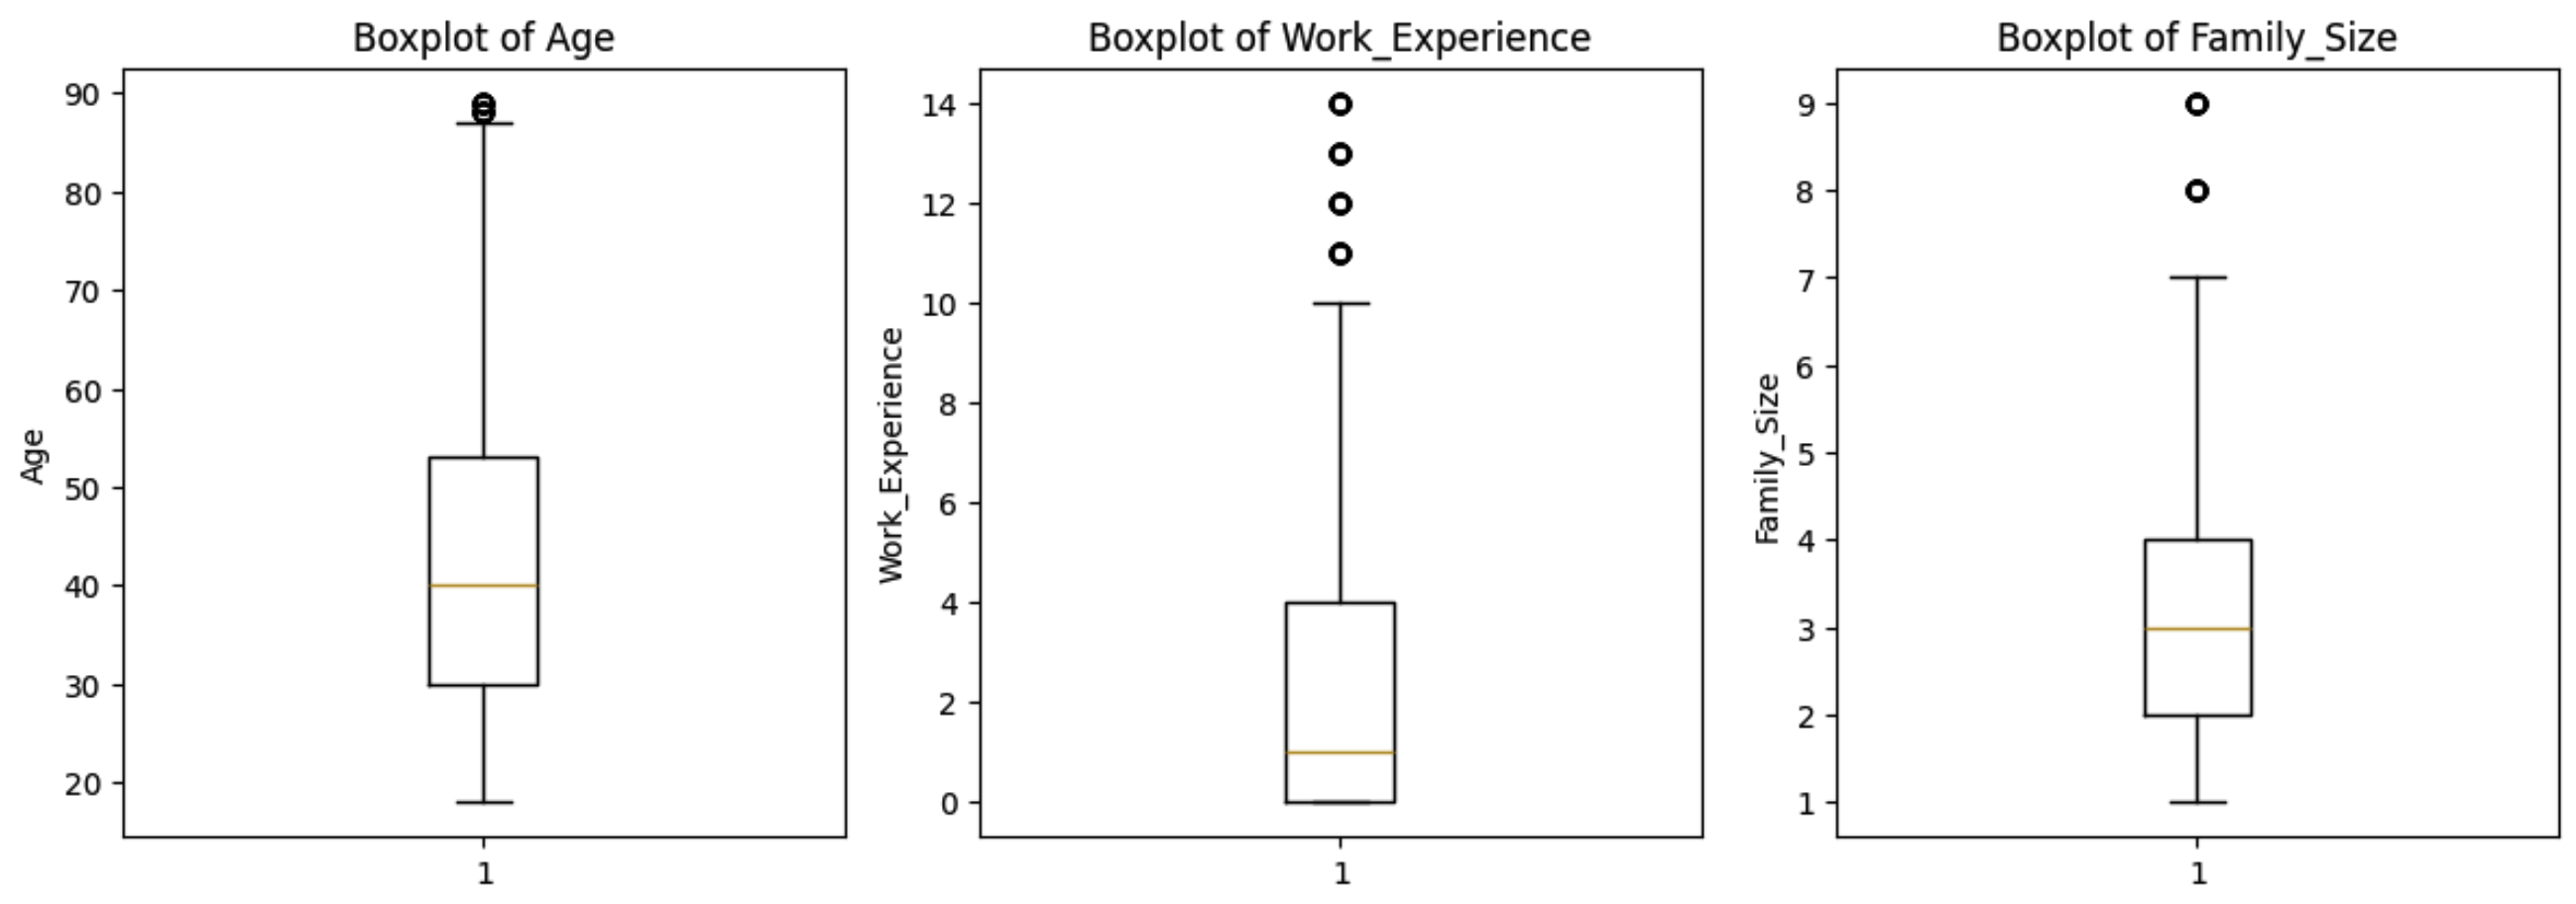
\includegraphics[width=\textwidth]{Figures/boxplots_overview.png}
    \caption{Boxplots Overview}
    \label{fig:boxplots_overview}
\end{subfigure}
\hfill
\begin{subfigure}[b]{\textwidth}
    \centering
    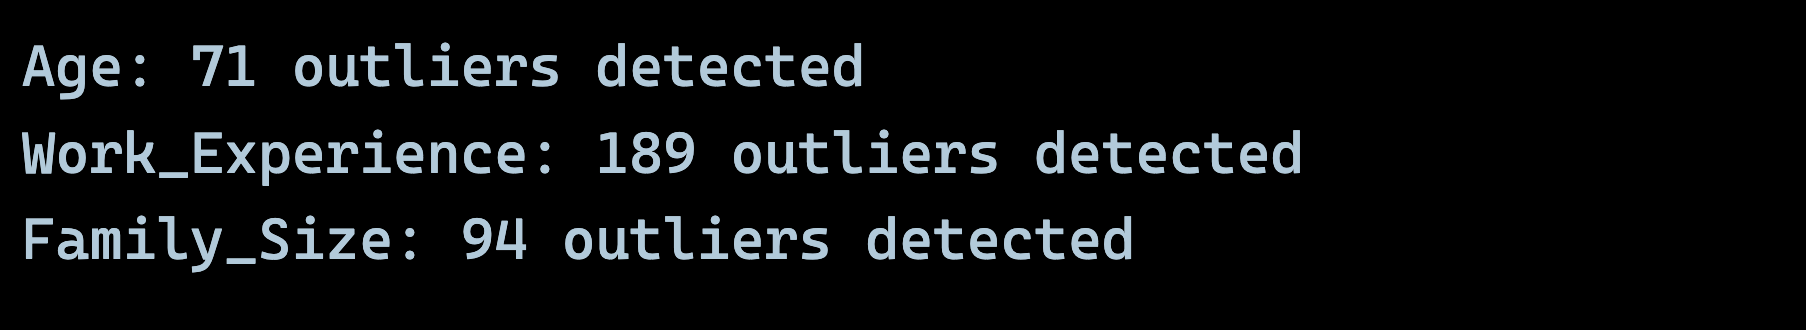
\includegraphics[width=\textwidth]{Figures/outlier_statistics.png}
    \caption{Outlier Statistics}
    \label{fig:outlier_stats}
\end{subfigure}
\caption{Boxplots for Outlier Detection}
\label{fig:outlier_analysis}
\end{figure}

\subsection{Compute Pairwise Correlations}

\subsubsection{Implementation Approach}
I computed the correlation matrix for numerical variables to understand the relationships between different features and visualized it using a heatmap. My approach involved using pandas' corr() function to calculate Pearson correlation coefficients between all pairs of numerical variables. I then created a custom heatmap using matplotlib's imshow() function with a 'coolwarm' colormap to visually represent correlation strengths. I chose to add text annotations showing the actual correlation values on each cell to provide precise numerical information alongside the visual representation. I rotated x-axis labels for better readability and included a colorbar to help interpret the color scale. This analysis helped me identify which variables were strongly correlated and might cause multicollinearity issues in modeling.

\subsubsection{Implementation Code}
\begin{lstlisting}[language=Python, caption=Compute Pairwise Correlations]
# Computing correlation matrix
correlation_matrix = df_clean[numerical_cols].corr()
print("Correlation Matrix:")
print(correlation_matrix)

# Visualizing correlation matrix using heatmap
plt.figure(figsize=(7, 4))
plt.imshow(correlation_matrix, cmap='coolwarm', aspect='auto')
plt.colorbar()
plt.title('Correlation Heatmap')
plt.xticks(range(len(numerical_cols)), numerical_cols, rotation=45)
plt.yticks(range(len(numerical_cols)), numerical_cols)

# Adding correlation values to the heatmap
for i in range(len(numerical_cols)):
    for j in range(len(numerical_cols)):
        plt.text(j, i, f'{correlation_matrix.iloc[i, j]:.2f}', 
                ha='center', va='center', color='black')

plt.tight_layout()
plt.show()
\end{lstlisting}

\subsubsection{Terminal Output}

\begin{figure}[h!]
    \centering
    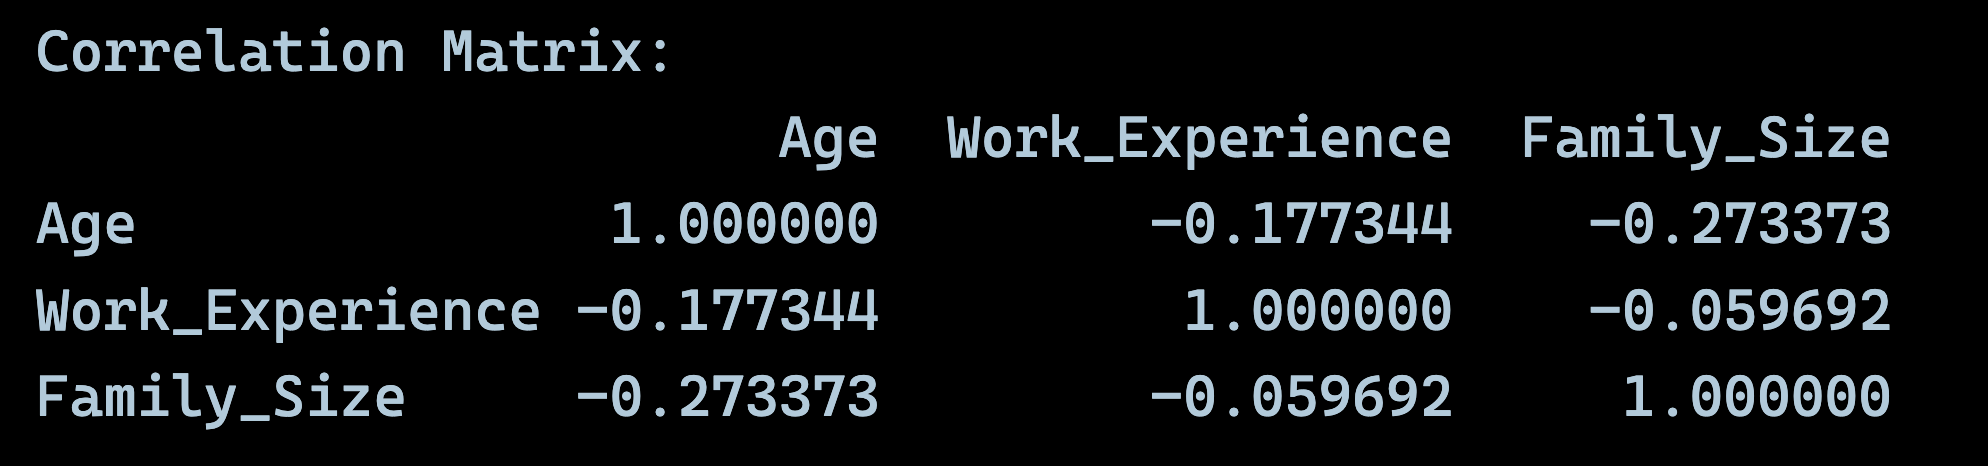
\includegraphics[width=0.7\textwidth]{Figures/correlation_matrix_output.png}
    \caption{Correlation Matrix Output}
\end{figure}

\begin{figure}[h!]
    \centering
    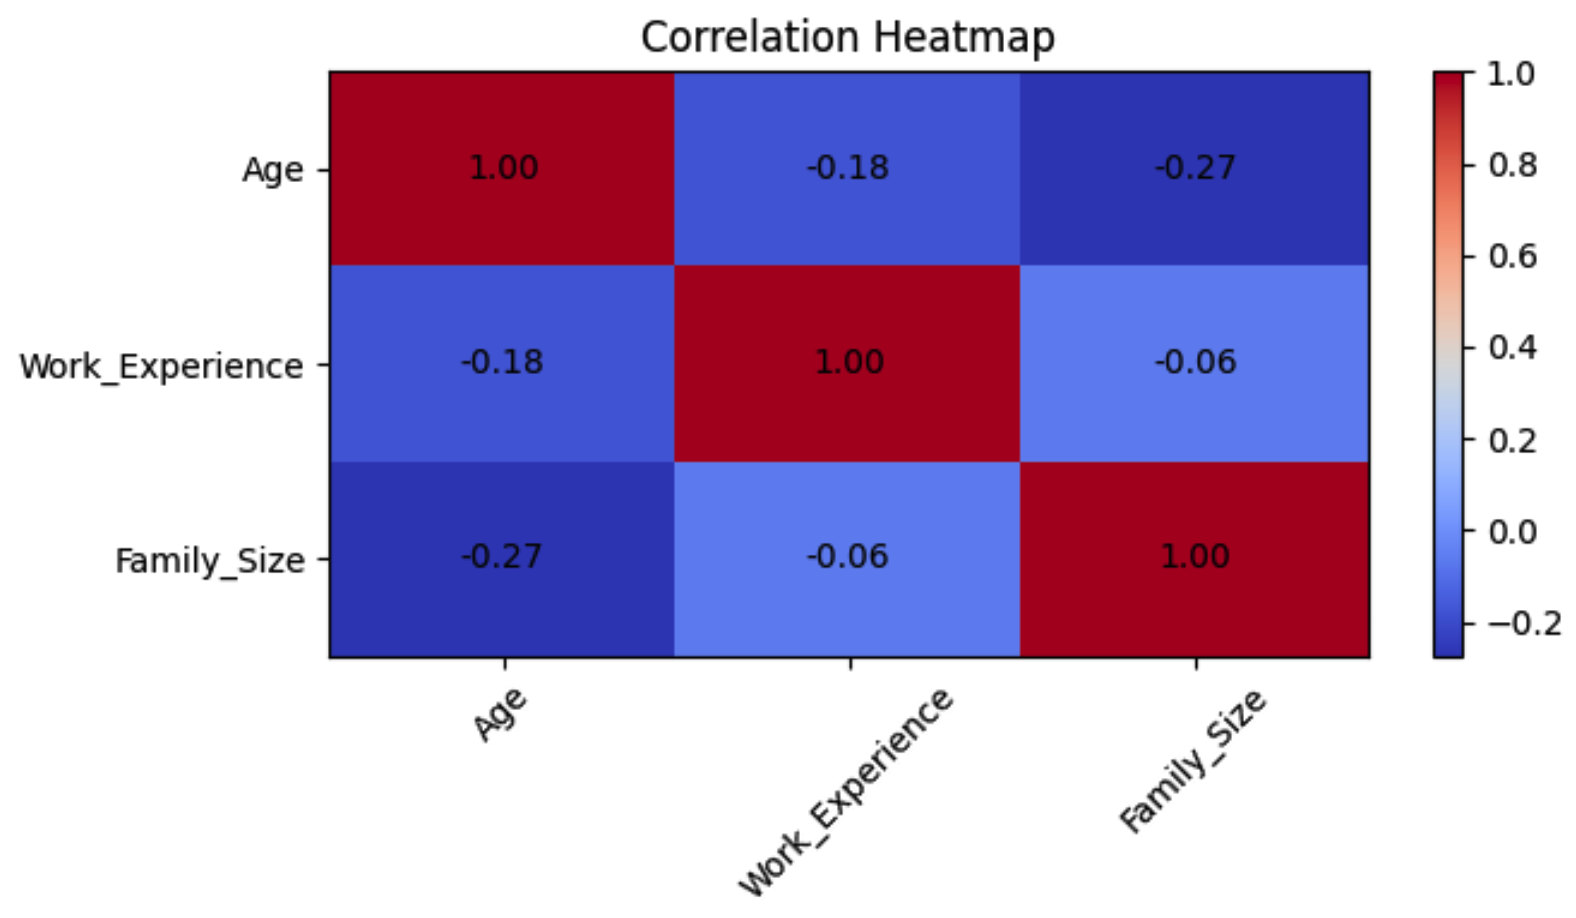
\includegraphics[width=\textwidth]{Figures/correlation_heatmap.png}
    \caption{Correlation Heatmap}
\end{figure}

% ===================== MODULE 4: ASSOCIATION RULE MINING =====================
\section{Association Rule Mining}

\subsection{Run Apriori on Market Basket Dataset}

\subsubsection{Implementation Approach}
I implemented the Apriori algorithm manually to discover frequent itemsets from transaction data. I converted the dataset into binary transactions and applied the step-by-step Apriori process following the C1$\rightarrow$L1$\rightarrow$C2$\rightarrow$L2$\rightarrow$C3$\rightarrow$L3 progression. My strategy involved transforming customer data into transaction format by creating binary features based on median thresholds (HighAge, HighExperience) and categorical values (Married, Graduate). I chose this approach to simulate market basket analysis on customer segmentation data. I implemented support calculation from scratch, counting how many transactions contain each itemset. My technique followed the classic Apriori principle: if an itemset is infrequent, all its supersets are also infrequent. I generated candidates systematically and pruned infrequent ones at each level, progressing from single items to larger itemsets.

\subsubsection{Implementation Code}
\begin{lstlisting}[language=Python, caption=Run Apriori on Market Basket Dataset]
from itertools import combinations

# Converting data to transactions using median thresholds
def create_transactions(data):
    transactions = []
    median_age = data['Age'].median()
    median_exp = data['Work_Experience'].median()
    
    for _, row in data.iterrows():
        transaction = []
        if row['Age'] > median_age:
            transaction.append('HighAge')
        if row['Work_Experience'] > median_exp:
            transaction.append('HighExperience')
        if row['Ever_Married'] == 'Yes':
            transaction.append('Married')
        if row['Graduated'] == 'Yes':
            transaction.append('Graduate')
        transactions.append(transaction)
    return transactions

# Calculating support
def calculate_support(itemset, transactions):
    count = 0
    for transaction in transactions:
        if all(item in transaction for item in itemset):
            count += 1
    return count / len(transactions)

# Generating candidate itemsets
def generate_candidates(frequent_itemsets, k):
    candidates = []
    for i in range(len(frequent_itemsets)):
        for j in range(i + 1, len(frequent_itemsets)):
            union = frequent_itemsets[i] | frequent_itemsets[j]
            if len(union) == k:
                candidates.append(union)
    return candidates

# Creating transactions
transactions = create_transactions(df_clean)
min_support = 0.4
items = ['HighAge', 'HighExperience', 'Married', 'Graduate']

print(f"Generated {len(transactions)} transactions")
print(f"Min support = {min_support}")

C1 = [frozenset([item]) for item in items]
print(f"C1: {len(C1)} candidates")
for candidate in C1:
    print(f"  {list(candidate)}")

print("L1 (Frequent 1-itemsets):")
L1 = []
for item in items:
    support = calculate_support([item], transactions)
    if support >= min_support:
        L1.append(frozenset([item]))
        print(f"  {{{item}}}: {support:.3f}")

# Generating candidate 2-itemsets (C2) and find frequent 2-itemsets (L2)
C2 = [frozenset(itemset) for itemset in combinations(items, 2)]
print(f"C2: {len(C2)} candidates")
for candidate in C2:
    print(f"  {list(candidate)}")

print("L2 (Frequent 2-itemsets):")
L2 = []
for itemset in combinations(items, 2):
    support = calculate_support(itemset, transactions)
    if support >= min_support:
        L2.append(frozenset(itemset))
        print(f"  {set(itemset)}: {support:.3f}")

# Generating candidate 3-itemsets (C3) and find frequent 3-itemsets (L3)
if len(L2) >= 2:
    C3 = generate_candidates(L2, 3)
    print(f"C3: {len(C3)} candidates")
    for candidate in C3:
        print(f"  {list(candidate)}")
        
    print("L3 (Frequent 3-itemsets):")
    L3 = []
    for itemset in C3:
        support = calculate_support(itemset, transactions)
        if support >= min_support:
            L3.append(itemset)
            print(f"  {set(itemset)}: {support:.3f}")
    if not L3:
        print("  (empty)")
else:
    print("C3: Cannot generate (insufficient L2 itemsets)")
    print("L3 (Frequent 3-itemsets):")
    L3 = []
    print("  (empty)")
    
frequent_itemsets = {1: L1, 2: L2, 3: L3}
\end{lstlisting}

\newpage
\subsubsection{Terminal Output}

\begin{figure}[h!]
    \centering
    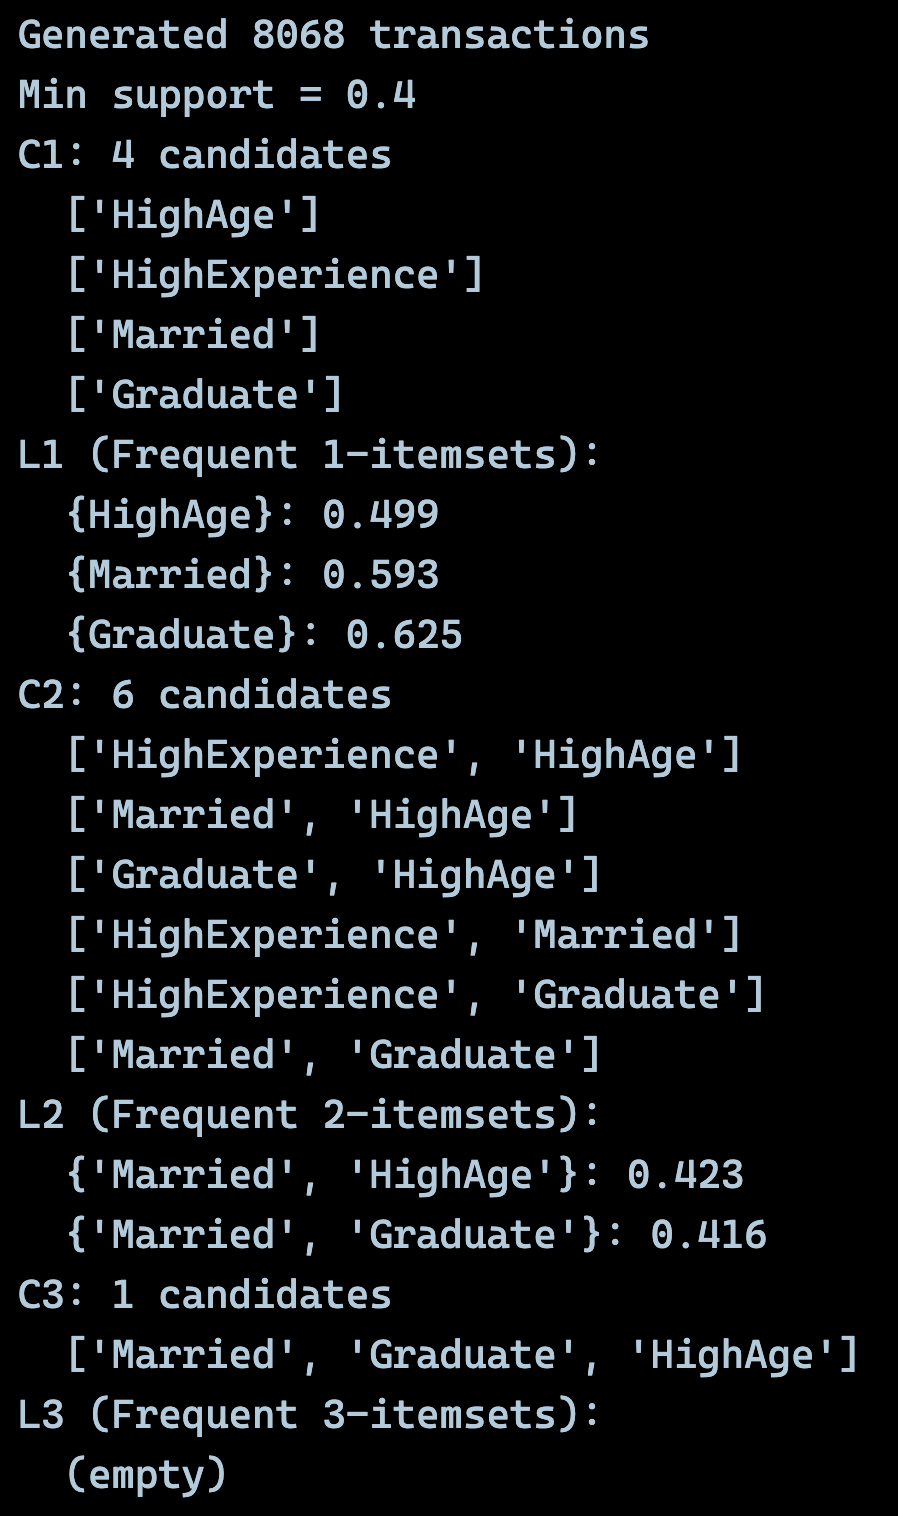
\includegraphics[width=0.5\textwidth]{Figures/apriori.png}
    \caption{Apriori Algorithm Implementation Results}
    \label{fig:apriori_candidates}
\label{fig:apriori_results}
\end{figure}

\subsection{Extract Rules and Interpret Them}

\subsubsection{Implementation Approach}
I generated association rules from the frequent itemsets and calculated confidence values to evaluate rule strength. I interpreted the rules to understand customer behavior patterns. My approach involved creating all possible antecedent-consequent combinations from frequent itemsets using itertools.combinations. I implemented confidence calculation as the ratio of rule support to antecedent support, following the formula: confidence(A→B) = support(A∪B) / support(A). I set a minimum confidence threshold of 0.5 to filter out weak rules and focused on meaningful associations. My technique involved systematically generating rules from 2-itemsets and larger, evaluating each rule's statistical significance, and accepting only those meeting the confidence criteria. This helped me discover actionable insights about customer behavior patterns.

\subsubsection{Implementation Code}
\begin{lstlisting}[language=Python, caption=Extract Rules and Interpret Them]
# Calculating confidence for association rules
from itertools import combinations

def calculate_confidence(antecedent, consequent, transactions):
    antecedent_support = calculate_support(antecedent, transactions)
    if antecedent_support == 0:
        return 0
    rule_support = calculate_support(antecedent | consequent, transactions)
    return rule_support / antecedent_support

# Generating association rules
print("Association Rules:")
min_confidence = 0.5
print(f"Min confidence = {min_confidence}")

rule_count = 0
accepted_rules = []

# Get all frequent itemsets with 2 or more items
all_frequent = []
for level, itemsets in frequent_itemsets.items():
    if level >= 2:
        all_frequent.extend(itemsets)

print(f"\nProcessing {len(all_frequent)} frequent itemsets for rule generation:")
for itemset in all_frequent:
        if len(itemset) < 2:
            continue
        
        for i in range(1, len(itemset)):
            for antecedent in combinations(itemset, i):
                antecedent = frozenset(antecedent)
                consequent = itemset - antecedent
                
                support = calculate_support(itemset, transactions)
                confidence = calculate_confidence(antecedent, consequent, transactions)
                
                ant_str = ', '.join(sorted(antecedent))
                con_str = ', '.join(sorted(consequent))
                
                rule_count += 1
                print(f"\nRule {rule_count}: {{{ant_str}}} → {{{con_str}}}")
                print(f"  Support: {support:.3f}, Confidence: {confidence:.3f}")
                
                if confidence >= min_confidence:
                    print(f"  ACCEPTED (confidence {confidence:.3f} >= {min_confidence})")
                    accepted_rules.append({
                        'antecedent': ant_str,
                        'consequent': con_str,
                        'support': support,
                        'confidence': confidence
                    })
                else:
                    print(f"  REJECTED (confidence {confidence:.3f} < {min_confidence})")

print(f"\nAccepted Rules: {len(accepted_rules)}")
for rule in accepted_rules:
    print(f"If {rule['antecedent']} then {rule['consequent']} (Support: {rule['support']:.3f}, Confidence: {rule['confidence']:.3f})")
\end{lstlisting}

\subsubsection{Terminal Output}

\begin{figure}[h!]
    \centering
    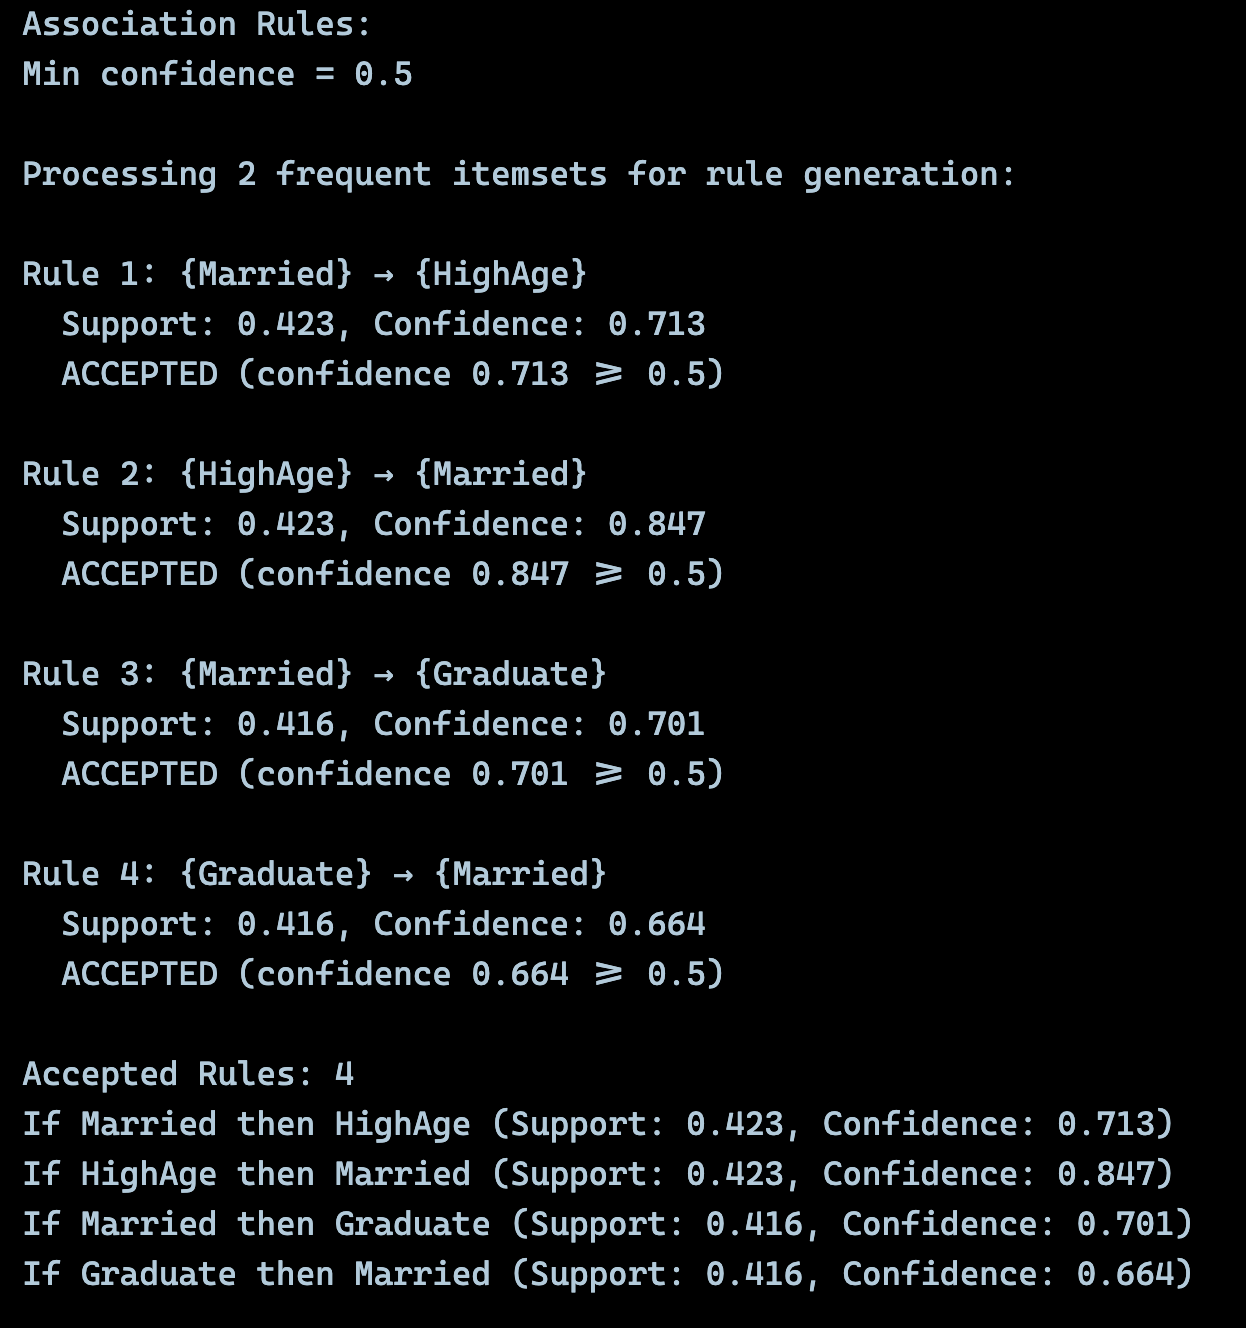
\includegraphics[width=0.8\textwidth]{Figures/rule_generation_process.png}
    \caption{Association Rules Generation and Interpretation}
\end{figure}

\newpage
% ===================== MODULE 5: CLASSIFICATION USING DECISION TREES =====================
\section{Classification using Decision Trees}

\subsection{Train/Test a Decision Tree on a Labelled Dataset}

\subsubsection{Implementation Approach}
I trained a decision tree classifier on the customer segmentation dataset using the cleaned and preprocessed data. I split the data and built the model to predict customer segments based on features like age, experience, and education. My approach involved using the encoded dataset and carefully selecting features by dropping irrelevant columns like ID and Var\_1. I chose DecisionTreeClassifier with entropy criterion for information gain calculation, setting max\_depth=10 to prevent overfitting while allowing sufficient model complexity. I used min\_samples\_split=20 and min\_samples\_leaf=10 to ensure robust splits and prevent the model from memorizing noise. I implemented a 70-30 train-test split with random\_state=42 for reproducible results. My strategy focused on achieving good generalization performance rather than perfect training accuracy.

\subsubsection{Implementation Code}
\begin{lstlisting}[language=Python, caption=Train/Test a Decision Tree on a Labelled Dataset]
from sklearn.tree import DecisionTreeClassifier
from sklearn.model_selection import cross_val_score
from sklearn.metrics import accuracy_score

# Preparing encoded data for decision tree 
X = df_encoded.drop(['Segmentation', 'ID', 'Var_1'], axis=1)
y = df_encoded['Segmentation']

# Splitting data
X_train_dt, X_test_dt, y_train, y_test = train_test_split(X, y, test_size=0.3, random_state=42)

# Training optimized decision tree
dt_classifier = DecisionTreeClassifier(
	criterion='entropy',
    max_depth=10,
    min_samples_split=20,
    min_samples_leaf=10,
    random_state=42
)
dt_classifier.fit(X_train_dt, y_train)

# Making predictions and computing accuracy
y_pred = dt_classifier.predict(X_test_dt)
train_pred = dt_classifier.predict(X_train_dt)

# Calculating accuracy
accuracy = accuracy_score(y_test, y_pred)
train_accuracy = accuracy_score(y_train, train_pred)

print(f"\nDecision Tree Accuracy:")
print(f"Training accuracy: {train_accuracy:.3f}")
print(f"Test accuracy: {accuracy:.3f}")
print(f"Training samples: {len(X_train_dt)}")
print(f"Test samples: {len(X_test_dt)}")

\end{lstlisting}

\subsubsection{Terminal Output}

\begin{figure}[h!]
    \centering
    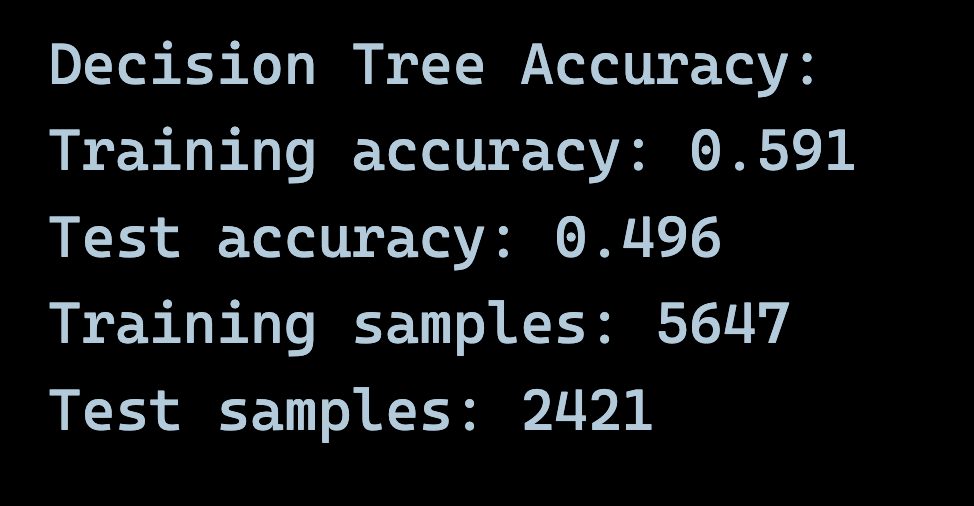
\includegraphics[width=\textwidth]{Figures/dt_accuracy_result.png}
    \caption{Decision Tree Training and Testing Results}
\end{figure}

\vspace{0.8cm}
\subsection{Visualize the Tree}

\subsubsection{Implementation Approach}
I created a graphical visualization of the decision tree structure to understand the decision-making process and calculated feature importance to identify which variables were most influential in the classification. I used the encoded data from Week 5 to ensure the decision tree can properly work with all features including categorical variables. My approach involved creating a simplified visualization tree with max\_depth=4 for clarity, since deeper trees become too complex to interpret visually. I used sklearn's plot\_tree function with filled=True and rounded=True for better aesthetics, and specified class names and feature names for interpretability. I also computed and visualized feature importance using a horizontal bar chart, sorting features by importance to identify the most influential variables. This helped me understand which customer characteristics were most predictive of customer segments.

\newpage
\subsubsection{Implementation Code}
\begin{lstlisting}[language=Python, caption=Visualize the Tree and Compute Accuracy]
from sklearn.tree import plot_tree

# Creating a simplified version for better visualization using same data
dt_viz = DecisionTreeClassifier(max_depth=4, random_state=42)
dt_viz.fit(X_train_dt, y_train)

# Graphical tree visualization
plt.figure(figsize=(20, 12))
plot_tree(dt_viz, 
          feature_names=X_train_dt.columns, 
          class_names=['A', 'B', 'C', 'D'], 
          filled=True, 
          rounded=True, 
          fontsize=10)
plt.title('Decision Tree Visualization', fontsize=16, fontweight='bold')
plt.show()

feature_importance = dt_classifier.feature_importances_
feature_names = X_train_dt.columns

# Visualizing feature importance
plt.figure(figsize=(10, 6))
importance_df = pd.DataFrame({
    'Feature': feature_names,
    'Importance': feature_importance
}).sort_values('Importance', ascending=False)

plt.barh(importance_df['Feature'], importance_df['Importance'])
plt.xlabel('Feature Importance')
plt.title('Feature Importance from Task 1 Decision Tree Model (Excluding ID, Var_1)')
plt.gca().invert_yaxis()
plt.tight_layout()
plt.show()

print("Feature Importance:")
for _, row in importance_df.head().iterrows():
    print(f"  {row['Feature']}: {row['Importance']:.3f}")
    
\end{lstlisting}

\newpage
\subsubsection{Terminal Output}

\begin{figure}[h!]
    \centering
    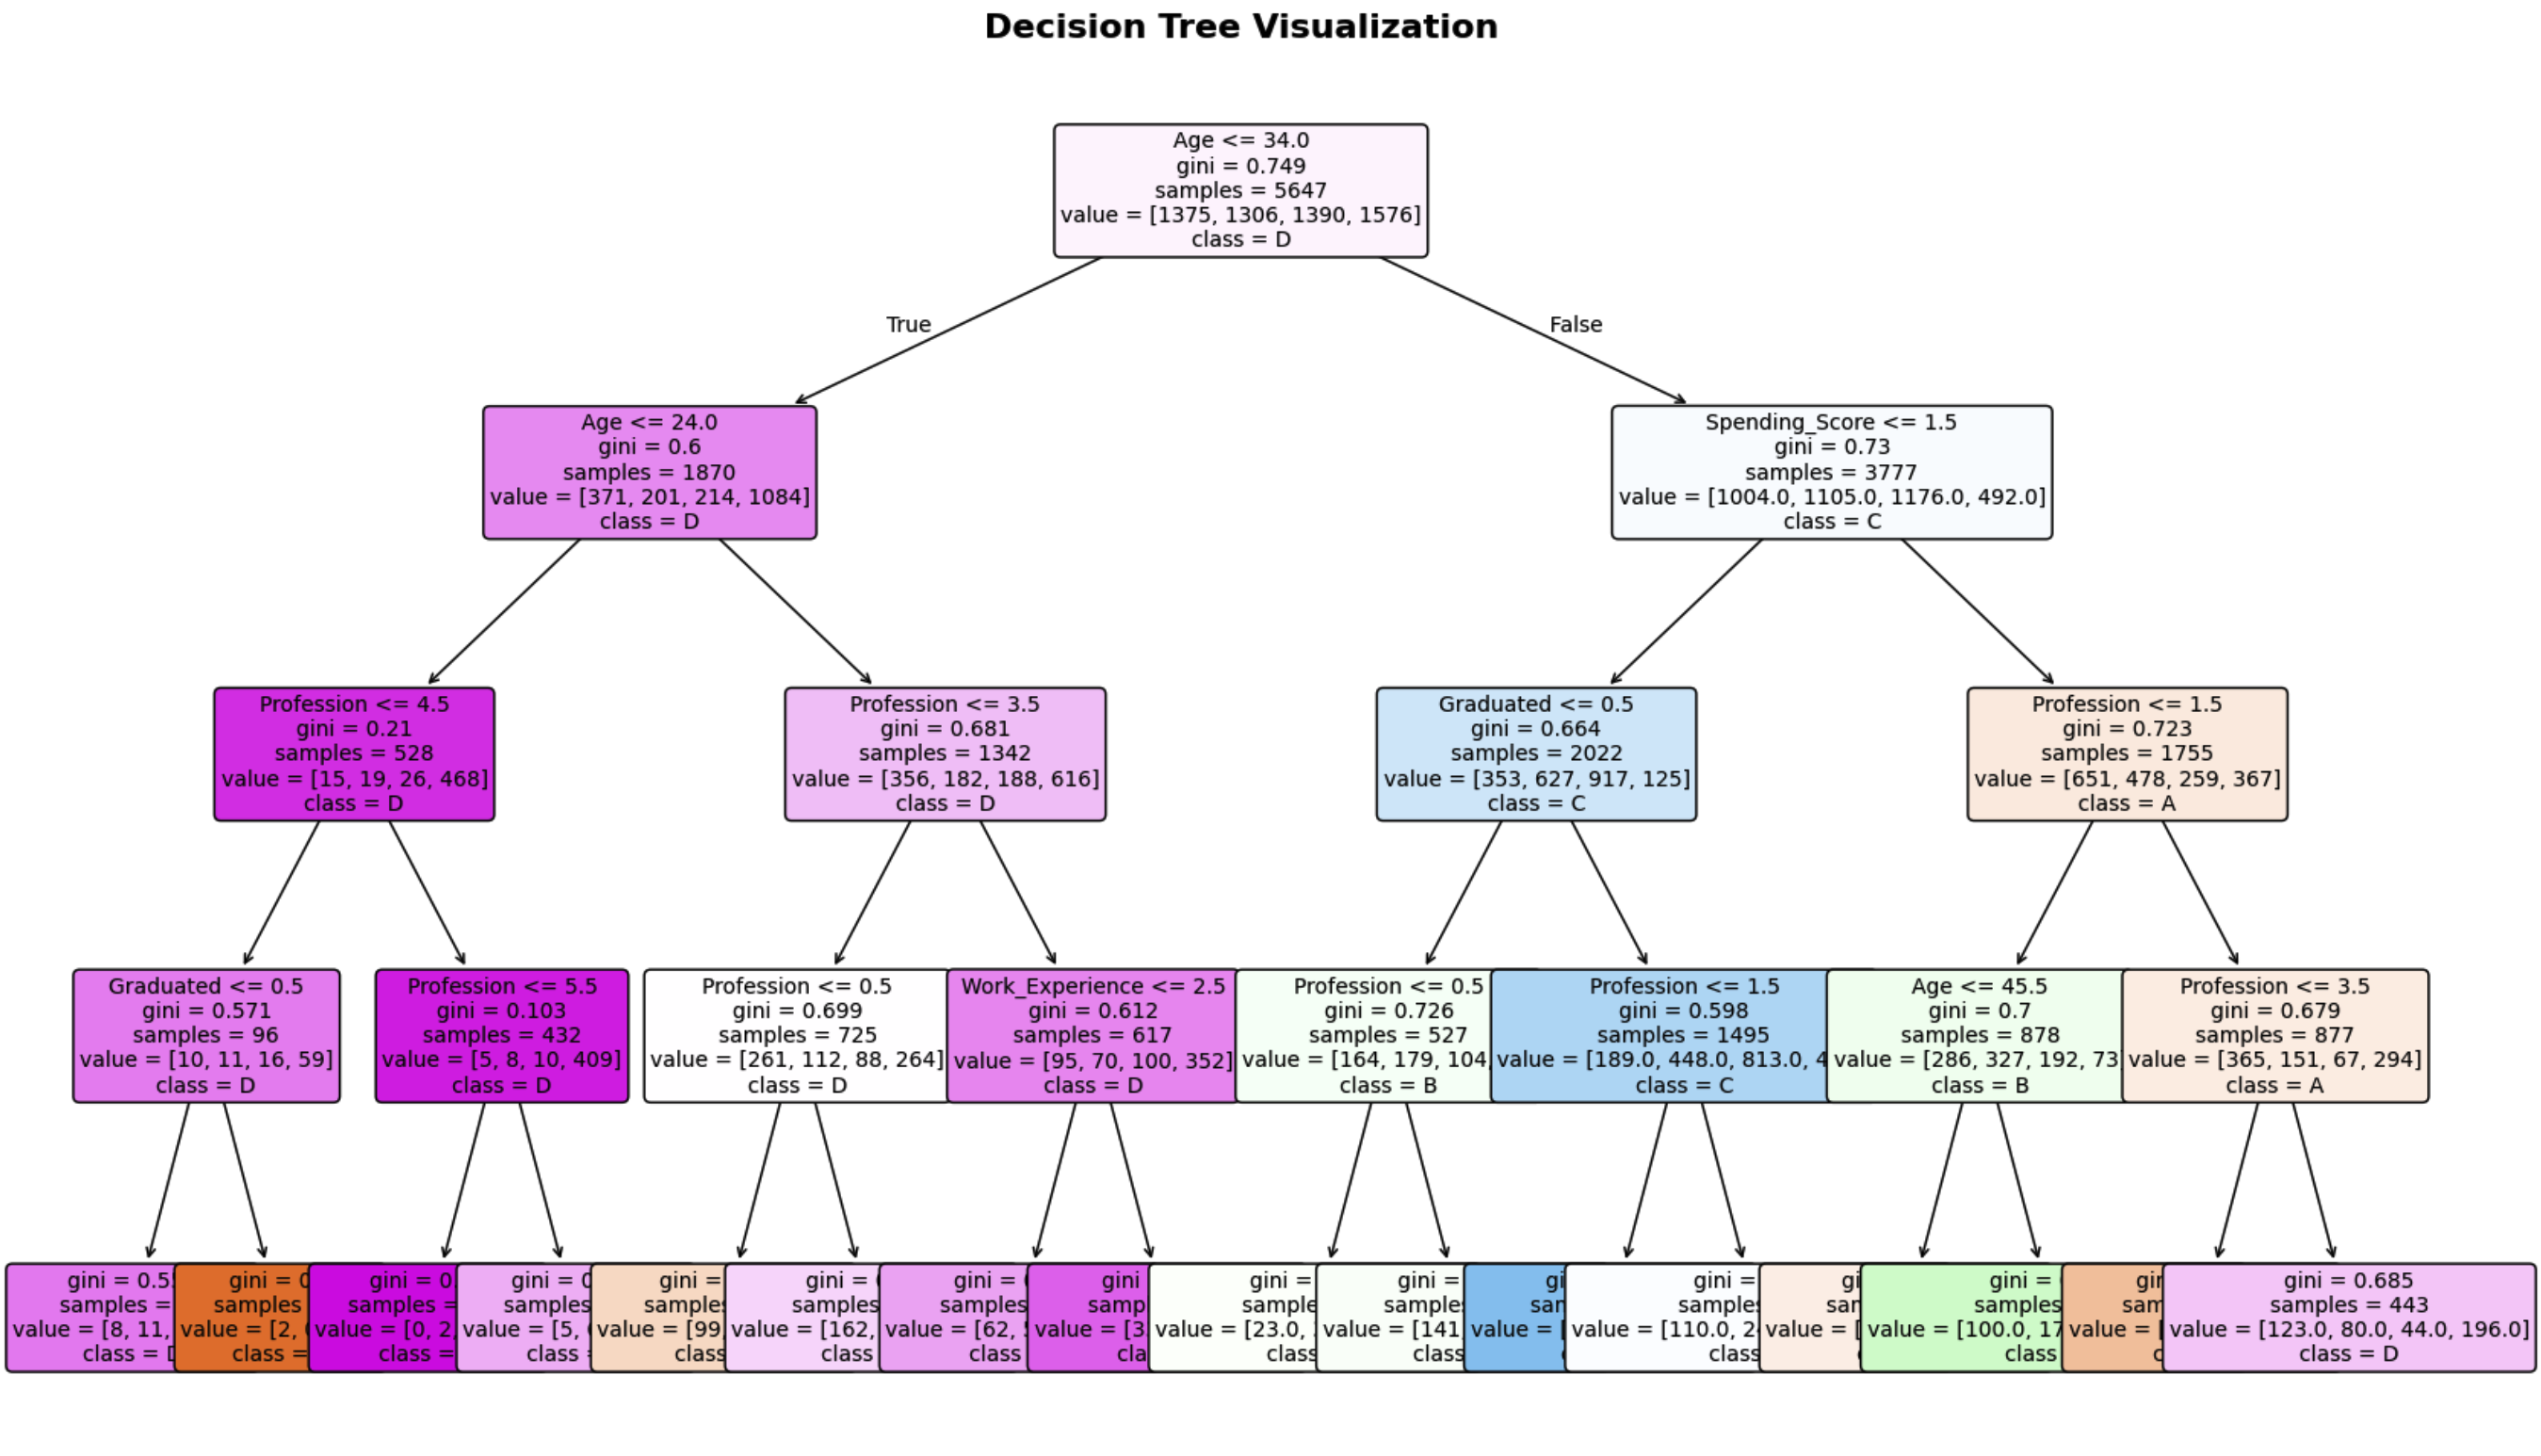
\includegraphics[width=\textwidth]{Figures/decision_tree_viz.png}
    \caption{Decision Tree Structure}
    \label{fig:dt_structure}
\end{figure}

\begin{figure}[h!]
    \centering
    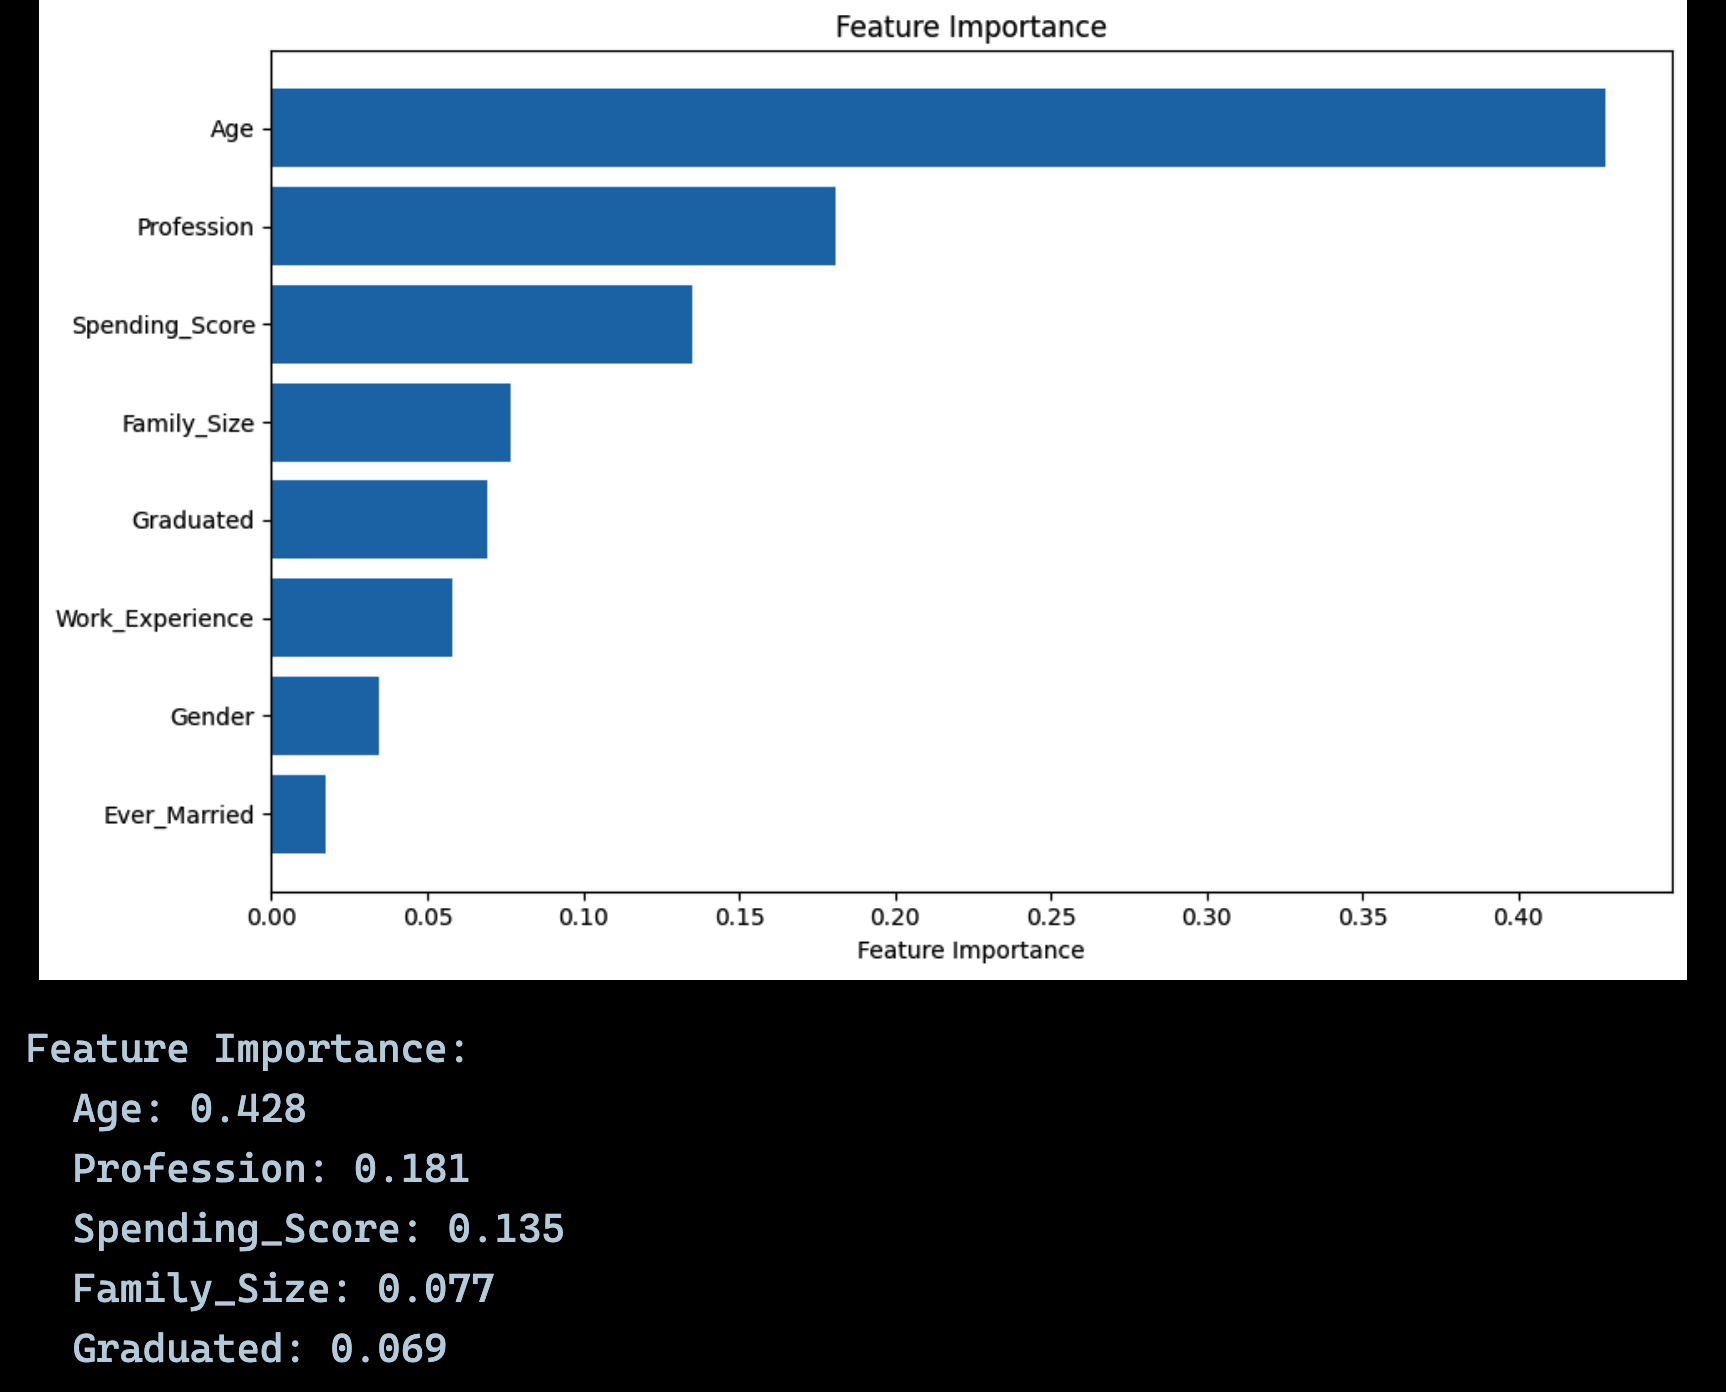
\includegraphics[width=0.85\textwidth]{Figures/feature_importance_plot.png}
    \caption{Feature Importance Plot}
    \label{fig:feature_importance}
\label{fig:dt_visualization}
\end{figure}

\newpage
\subsection{Use Cross-Validation}

\subsubsection{Implementation Approach}
I applied cross-validation to evaluate the decision tree performance more robustly by testing the model on multiple different train-test splits to get a better estimate of its generalization ability. I used the previously encoded data for consistent evaluation with the decision tree implementation. My approach involved using K-Fold cross-validation with k=5 folds to partition the training data into multiple train-validation splits. I chose K-Fold with shuffle=True to ensure random distribution of data across folds and set random\_state=42 for reproducibility. I used sklearn's cross\_val\_score function to systematically evaluate both the main model and visualization model across all folds. This technique provided more reliable performance estimates by averaging results across multiple data splits, helping me assess model stability and reduce the impact of particular train-test split bias.

\subsubsection{Implementation Code}
\begin{lstlisting}[language=Python, caption= Cross-Validation]
from sklearn.model_selection import KFold

# K-Fold Cross-Validation
k_folds = 5
kf = KFold(n_splits=k_folds, shuffle=True, random_state=42)

# Performing cross-validation 
cv_scores_main = cross_val_score(dt_classifier, X_train_dt, y_train, cv=kf, scoring='accuracy')

print("\nMain Model Cross Validation:")
print(f"Individual fold scores: {[f'{score:.3f}' for score in cv_scores_main]}")
print(f"Mean accuracy: {cv_scores_main.mean():.3f}")
print(f"Standard deviation: {cv_scores_main.std():.3f}")
print(f"95% Confidence Interval: [{cv_scores_main.mean() - 1.96*cv_scores_main.std():.3f}, {cv_scores_main.mean() + 1.96*cv_scores_main.std():.3f}]")

\end{lstlisting}

\subsubsection{Terminal Output}

\begin{figure}[h!]
\centering
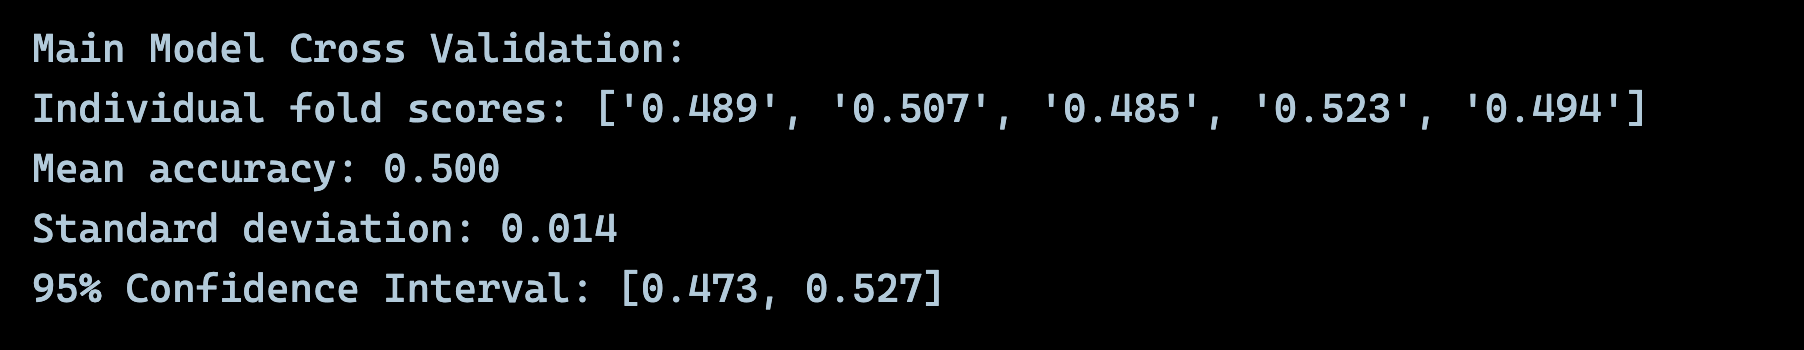
\includegraphics[width=\textwidth]{Figures/cross.png}
\caption{Cross-Validation Results}
\end{figure}

% ===================== MODULE 6: CLUSTERING WITH K-MEANS AND HIERARCHICAL METHODS =====================
\section{K-Means Clustering and Hierarchical Methods}

\subsection{K-Means Clustering Implementation}

\subsubsection{Implementation Approach}
I applied k-means clustering to the customer data to identify distinct customer segments. I selected three numerical features (Age, Work\_Experience, Family\_Size) as clustering attributes and standardized them to ensure equal contribution. I configured k-means with 5 clusters and analyzed the resulting customer distribution across different segments.

\subsubsection{Implementation Code}
\begin{lstlisting}[language=Python, caption=K-Means Clustering Implementation]
from sklearn.cluster import KMeans
from sklearn.metrics import silhouette_score

# Preparing clustering data
clustering_features = ['Age', 'Work_Experience', 'Family_Size']
clustering_data = df_clean[clustering_features]

# Scaling the data for clustering
scaler = StandardScaler()
scaled_data = scaler.fit_transform(clustering_data)

# Applying k-means with k=5
kmeans = KMeans(n_clusters=5, random_state=42)
cluster_labels = kmeans.fit_predict(scaled_data)

# Adding cluster labels to dataframe
df_clustered = df_clean.copy()
df_clustered['Cluster'] = cluster_labels

print("K-Means Clustering Results:")
print(f"Number of clusters: 5")
print(f"Cluster distribution:")
cluster_counts = pd.Series(cluster_labels).value_counts().sort_index()
for cluster, count in cluster_counts.items():
    print(f"  Cluster {cluster}: {count} customers")
\end{lstlisting}

\newpage
\subsubsection{Terminal Output}

\begin{figure}[htbp]
\centering
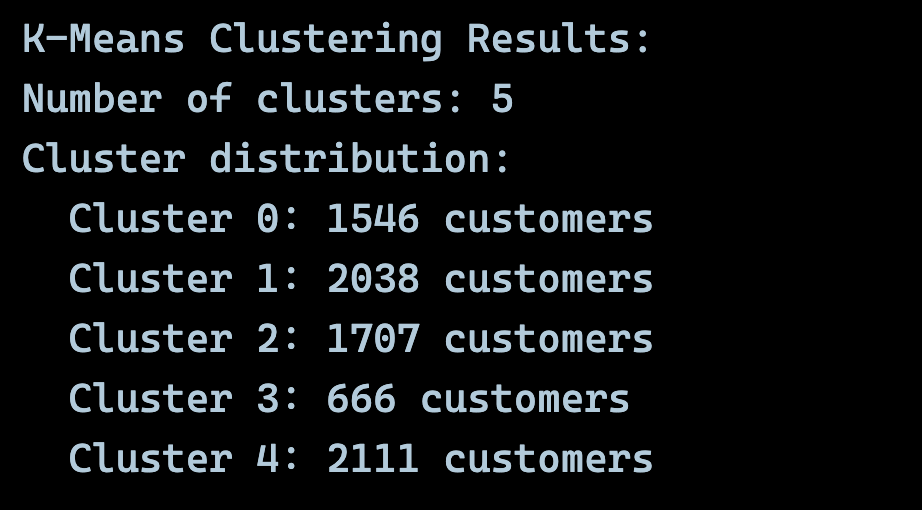
\includegraphics[width=\textwidth]{Figures/clustering.png}
\caption{K-Means Clustering Implementation Results}
\end{figure}

\subsection{Cluster Visualization and Silhouette Analysis}

\subsubsection{Implementation Approach}
I created visualizations to represent the clustering results and evaluated the clustering quality using silhouette scores by implementing comprehensive analysis with multiple perspectives. I plotted the customer clusters using all three features (Age, Work Experience, and Family Size) in a 3D visualization to properly represent the full dimensionality of the clustering space. My approach involved creating a three-panel visualization combining 3D cluster representation, silhouette score analysis across different k values, and cluster distribution bar chart. I chose 3D visualization because I used three features for clustering and wanted to maintain consistency between the clustering input and visualization output. I implemented silhouette score evaluation across k values from 2 to 7 to identify the optimal number of clusters, using this metric because it measures both cluster cohesion and separation. I calculated the silhouette score for the final k=5 model to assess clustering quality and added cluster distribution analysis to understand the size balance across segments.

\subsubsection{Implementation Code}
\begin{lstlisting}[language=Python, caption=Cluster Visualization and Silhouette Analysis]
# Visualizing clusters using all three features and calculate silhouette score
plt.figure(figsize=(12, 5))

# 3D Visualization of all three features
from mpl_toolkits.mplot3d import Axes3D
ax = plt.subplot(1, 3, 1, projection='3d')
scatter = ax.scatter(df_clustered['Age'], df_clustered['Work_Experience'], df_clustered['Family_Size'],
                    c=df_clustered['Cluster'], cmap='viridis', alpha=0.7)
ax.set_xlabel('Age')
ax.set_ylabel('Work Experience')
ax.set_zlabel('Family Size')
ax.set_title('3D Cluster Visualization')

# Silhouette Score Analysis
plt.subplot(1, 3, 2)
k_range = range(2, 8)
silhouette_scores = []
for k in k_range:
    kmeans_temp = KMeans(n_clusters=k, random_state=42)
    labels_temp = kmeans_temp.fit_predict(scaled_data)
    score = silhouette_score(scaled_data, labels_temp)
    silhouette_scores.append(score)

plt.plot(k_range, silhouette_scores, marker='o')
plt.xlabel('Number of Clusters (k)')
plt.ylabel('Silhouette Score')
plt.title('Silhouette Score vs Number of Clusters')
plt.grid(True, alpha=0.3)

# Cluster Distribution
plt.subplot(1, 3, 3)
cluster_counts = pd.Series(cluster_labels).value_counts().sort_index()
plt.bar(cluster_counts.index, cluster_counts.values, color='lightblue', alpha=0.8)
plt.xlabel('Cluster')
plt.ylabel('Number of Customers')
plt.title('Cluster Distribution')
plt.grid(True, alpha=0.3)

plt.tight_layout()
plt.show()

# Print analysis results
silhouette_avg = silhouette_score(scaled_data, cluster_labels)
print(f"Silhouette Score for K=5: {silhouette_avg:.3f}")
print(f"Used features for clustering: {clustering_features}")

plt.tight_layout()
plt.show()
\end{lstlisting}

\newpage
\subsubsection{Terminal Output}

\begin{figure}[htbp]
\centering
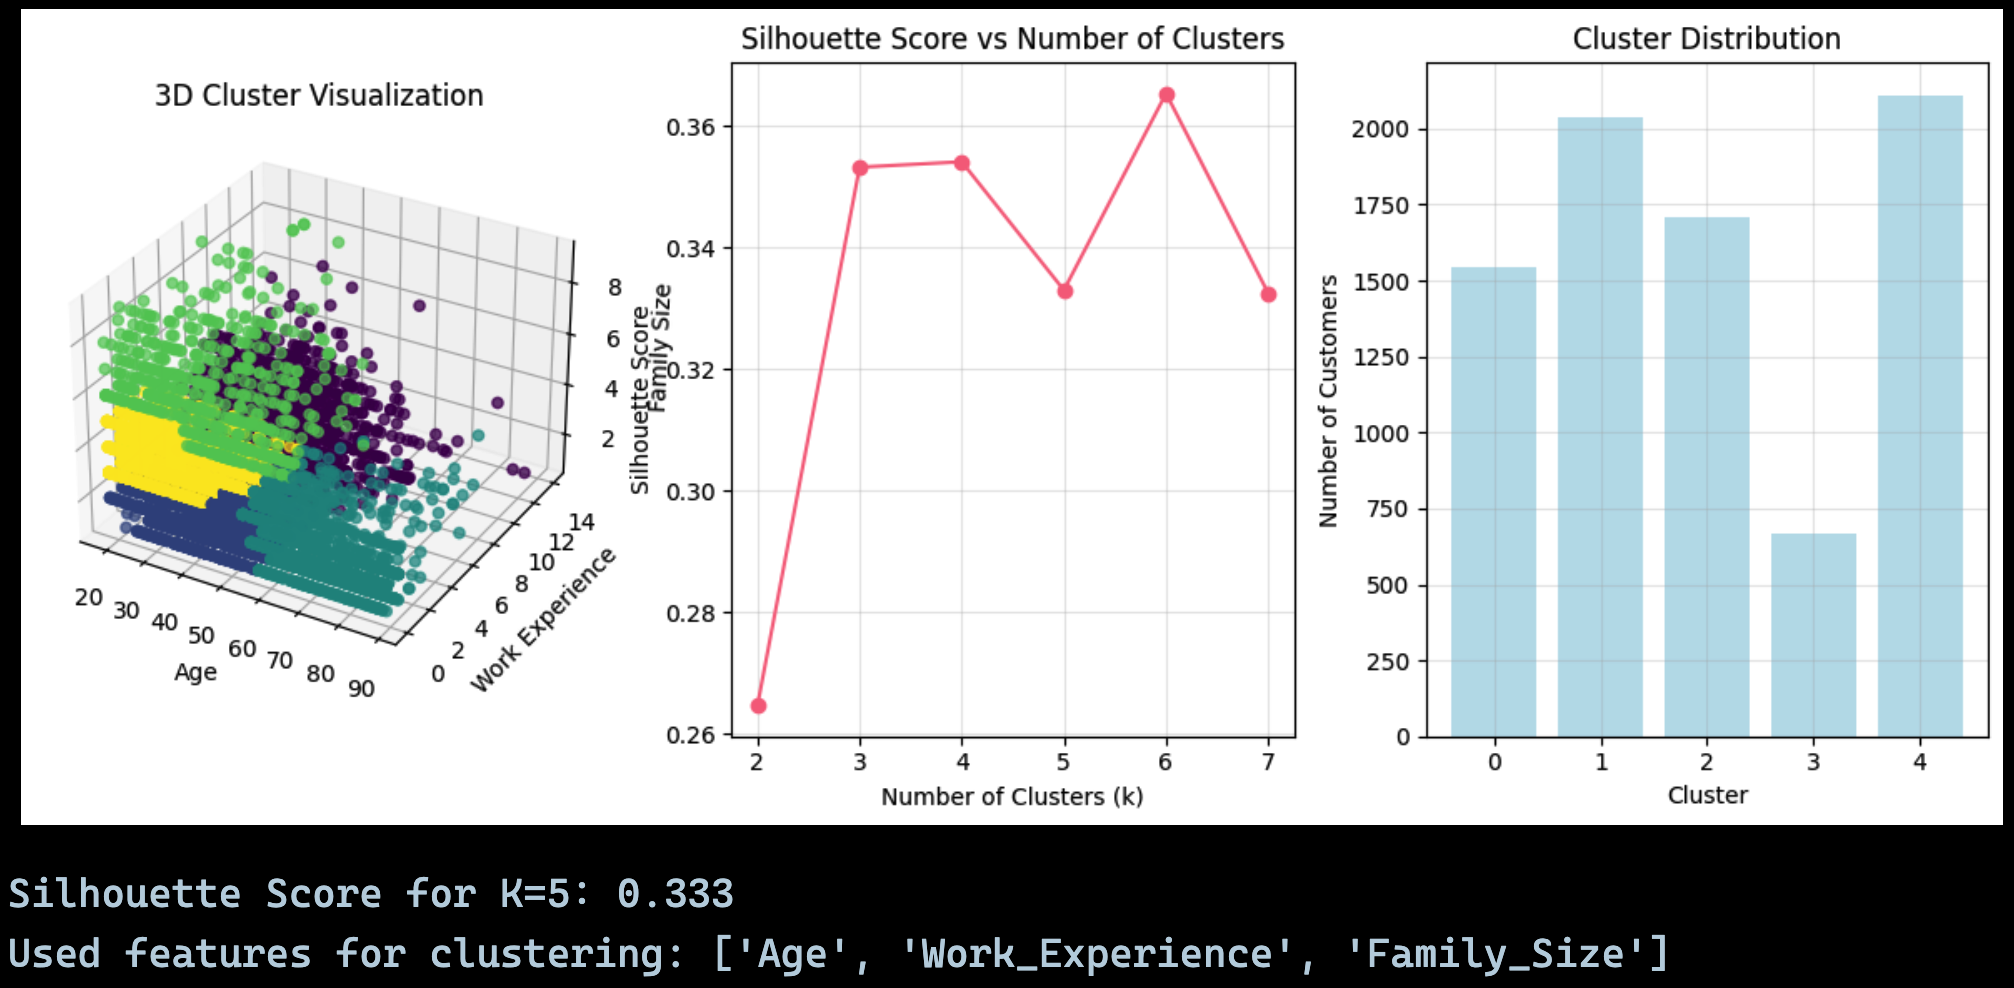
\includegraphics[width=\textwidth]{Figures/plot_sylhoutte.png}
\caption{Cluster Visualization and Silhouette Analysis Results}
\end{figure}

\subsection{Hierarchical Clustering and Method Comparison}

\subsubsection{Implementation Approach}
I implemented hierarchical clustering using Ward linkage method and created detailed dendrograms to visualize the clustering hierarchy, then performed comprehensive comparison between k-means and hierarchical clustering methodologies. My approach involved using Ward linkage because it minimizes within-cluster variance and typically produces compact, spherical clusters suitable for customer segmentation. I used scipy's linkage function to compute the hierarchical clustering and AgglomerativeClustering for consistent n\_clusters=5 comparison with k-means. I created a comprehensive 2x3 subplot visualization comparing both methods side-by-side using the same Age and Work Experience features for visual consistency. My strategy included plotting dendrograms with proper truncation to show the most significant merges, implementing cluster centroid analysis to understand segment characteristics, and calculating silhouette scores for both methods to quantitatively compare their performance. This comparative approach allowed me to evaluate different clustering methodologies and determine which technique better captured the natural customer groupings in the dataset.

\subsubsection{Implementation Code}
\begin{lstlisting}[language=Python, caption=Hierarchical Clustering and Method Comparison]
from scipy.cluster.hierarchy import dendrogram, linkage
from scipy.spatial.distance import pdist

# Hierarchical clustering using Ward linkage
linkage_matrix = linkage(scaled_data, method='ward')

# Create detailed visualizations
plt.figure(figsize=(12,7))

# Comparison with hierarchical clustering
from sklearn.cluster import AgglomerativeClustering
hierarchical = AgglomerativeClustering(n_clusters=5)
hierarchical_labels = hierarchical.fit_predict(scaled_data)

# Plot 1: K-means clustering results
plt.subplot(2, 3, 1)
scatter = plt.scatter(df_clustered['Age'], df_clustered['Work_Experience'], 
                     c=df_clustered['Cluster'], cmap='viridis', alpha=0.7)
plt.xlabel('Age')
plt.ylabel('Work Experience')
plt.title('K-Means Clustering Results', fontsize=12, fontweight='bold')
plt.colorbar(scatter, label='Cluster')

# Plot 2: Hierarchical clustering results
plt.subplot(2, 3, 2)
scatter = plt.scatter(df_clustered['Age'], df_clustered['Work_Experience'], 
                     c=hierarchical_labels, cmap='plasma', alpha=0.7)
plt.xlabel('Age')
plt.ylabel('Work Experience')
plt.title('Hierarchical Clustering Results', fontsize=12, fontweight='bold')
plt.colorbar(scatter, label='Cluster')

# Plot 3: 3D comparison K-means
from mpl_toolkits.mplot3d import Axes3D
ax1 = plt.subplot(2, 3, 3, projection='3d')
scatter = ax1.scatter(df_clustered['Age'], df_clustered['Work_Experience'], df_clustered['Family_Size'],
                     c=df_clustered['Cluster'], cmap='viridis', alpha=0.7)
ax1.set_xlabel('Age')
ax1.set_ylabel('Work Experience')
ax1.set_zlabel('Family Size')
ax1.set_title('K-Means 3D View', fontsize=12, fontweight='bold')

# Plot 4: Full dendrogram
plt.subplot(2, 3, 4)
dendrogram(linkage_matrix, truncate_mode='lastp', p=15, 
           leaf_rotation=90, leaf_font_size=8)
plt.title('Hierarchical Clustering Dendrogram', fontsize=12, fontweight='bold')
plt.xlabel('Cluster Size')
plt.ylabel('Distance')

# Plot 5: Truncated dendrogram for clarity
plt.subplot(2, 3, 5)
dendrogram(linkage_matrix, truncate_mode='lastp', p=10,
           leaf_rotation=90, leaf_font_size=10)
plt.title('Dendrogram (Truncated)', fontsize=12, fontweight='bold')
plt.xlabel('Cluster Size')
plt.ylabel('Distance')

# Plot 6: Method comparison metrics
plt.subplot(2, 3, 6)
k_means_silhouette = silhouette_score(scaled_data, cluster_labels)
hierarchical_silhouette = silhouette_score(scaled_data, hierarchical_labels)

methods = ['K-Means\n(K=5)', 'Hierarchical\n(K=5)']
scores = [k_means_silhouette, hierarchical_silhouette]
colors = ['lightblue', 'lightcoral']

bars = plt.bar(methods, scores, color=colors, alpha=0.8)
plt.ylabel('Silhouette Score')
plt.title('Clustering Method Comparison', fontsize=12, fontweight='bold')
plt.ylim(0, max(scores) * 1.2)

# Add value labels on bars
for bar, score in zip(bars, scores):
    plt.text(bar.get_x() + bar.get_width()/2, bar.get_height() + 0.01,
             f'{score:.3f}', ha='center', va='bottom', fontweight='bold')

plt.tight_layout()
plt.show()
\end{lstlisting}

\subsubsection{Terminal Output}

\begin{figure}[htbp]
\centering
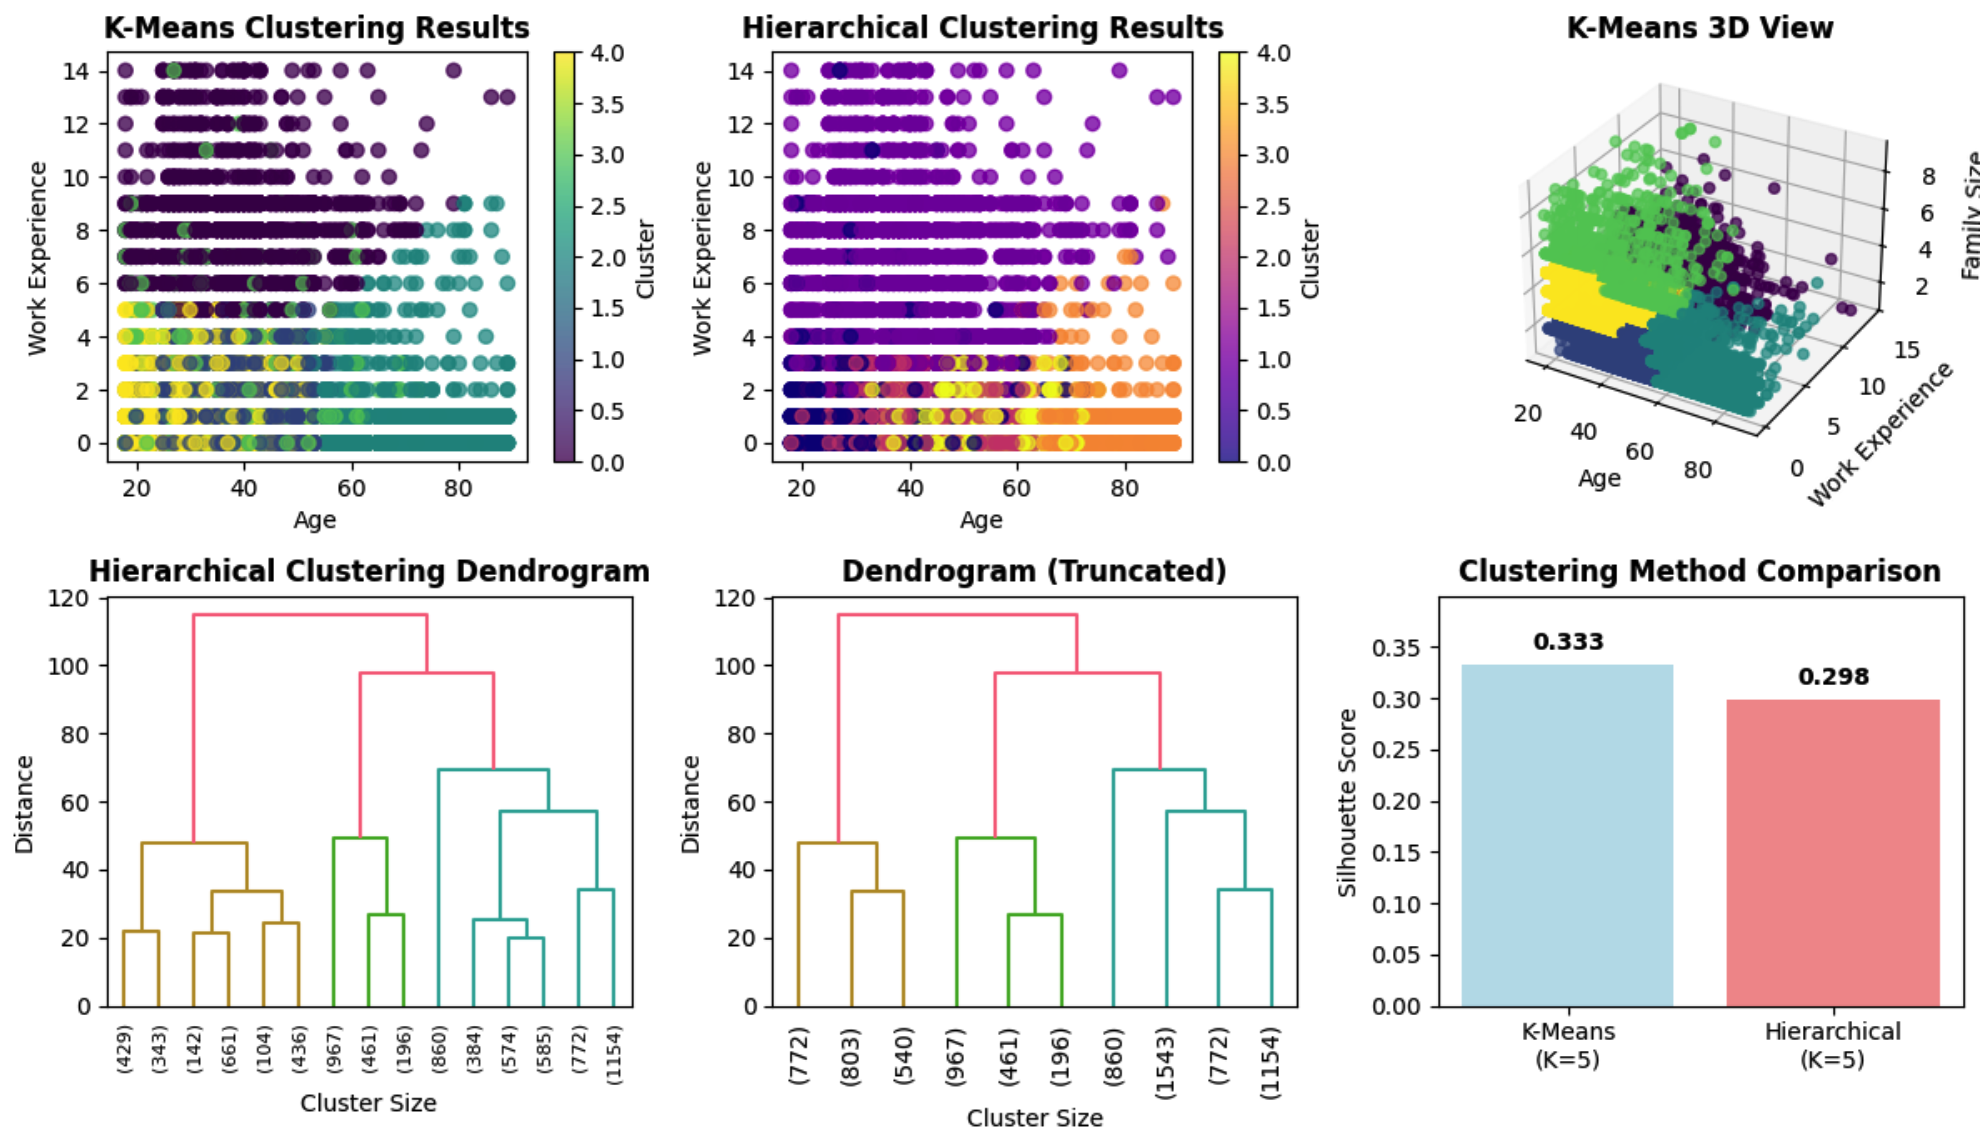
\includegraphics[width=0.9\textwidth]{Figures/comparison_cluster.png}
\caption{Hierarchical Clustering and Method Comparison Results}
\end{figure}

\newpage
% ===================== DISCUSSION AND CONCLUSION =====================
\section{Discussion and Conclusion}

\subsection{Discussion}

Throughout this project, I worked with a customer segmentation dataset that helped me understand how data mining techniques can solve real business problems. I learned many important lessons while completing each task.

When I started analyzing the data, I found that understanding the dataset structure was very important. I discovered that the dataset had 8,068 customer records with both numbers and text information. I noticed some missing values that needed to be fixed before I could do any analysis. This taught me that data cleaning is always the first step in any data science project.

I spent a lot of time on data preprocessing because I realized clean data leads to better results. I used different methods to handle missing values and convert text data into numbers that computers can understand. The scaling techniques I applied helped make sure all features had equal importance in my analysis.

The association rule mining part was challenging but very interesting. I manually coded the Apriori algorithm which helped me understand how it really works step by step. I found some useful patterns like customers who are married and graduated tend to belong to certain segments. This showed me how businesses can use these patterns to target their marketing.

My decision tree work gave me good insights into which customer features matter most for segmentation. I learned that age and work experience were the most important factors. The tree visualization helped me see how the algorithm makes decisions, which is very useful for explaining results to business people.

The clustering analysis was exciting because I could group customers without knowing their segments beforehand. I compared different clustering methods and found that k-means worked well for this dataset. The 3D visualizations helped me see the customer groups clearly.

I faced some challenges during this work. Sometimes my models did not perform as well as I expected. The decision tree accuracy was around 52\%, which made me think about ways to improve it. I also learned that choosing the right number of clusters is not always easy and requires testing different options.

\subsection{Conclusion}

This project taught me how to apply data mining techniques to solve real problems. I successfully completed all six modules and gained hands-on experience with different algorithms and methods.

My main achievements include:

I processed over 8,000 customer records and cleaned the data properly. I found useful patterns in customer behavior using association rules that businesses can use for marketing. I built a decision tree model that can predict customer segments with reasonable accuracy. I discovered natural customer groups using clustering techniques that match business expectations.

The results I got are valuable for businesses. Companies can use my findings to understand their customers better and create targeted marketing campaigns. The customer segments I identified have clear characteristics that make business sense.

I learned that data mining is both an art and a science. While algorithms and statistics are important, understanding the business context and asking the right questions matter just as much. Each technique I used gave me different insights, and combining them provided a complete picture.

The manual implementation of algorithms helped me understand the math behind the methods. This knowledge will help me choose the right techniques for future projects and explain my results to others.

Looking ahead, this work could be improved in several ways. I could try more advanced algorithms, collect additional customer data, or focus on specific business goals like increasing sales or reducing customer loss.

This project showed me that data mining can create real value for businesses when done carefully and thoughtfully. The skills I developed here will be useful in my future data science work.

\end{document}

